%!TEX spellcheck = en-US
%\documentclass[journal]{IEEEtran}
\documentclass[11pt,onecolumn,journal]{IEEEtran}
%
% If IEEEtran.cls has not been installed into the LaTeX system files,
% manually specify the path to it like:
% \documentclass[journal]{../sty/IEEEtran}

\usepackage[section]{placeins}

\usepackage{makecell}

\usepackage{graphicx, amssymb, amsmath,algorithm}
\graphicspath{{./fig/}}
\DeclareGraphicsExtensions{.pdf,.jpg,.jpeg,.png}
\usepackage{latexsym}
\usepackage{amsfonts}
\usepackage{amsopn}
%\newcommand{\argmax}{\operatornamewithlimits{argmax}}
%\newcommand{\argmin}{\operatornamewithlimits{argmin}} \newcommand{\comment}[1]{}
% \newcommand{\min}{\operatornamewithlimits{min}} \newcommand{\comment}[1]{}
\usepackage[dvipsnames]{xcolor}
\usepackage[normalem]{ulem}
\usepackage{enumitem}
\usepackage{parskip}

\usepackage{algorithmic}
\usepackage{calc}
\usepackage{array}
\usepackage{tabularx}
\usepackage{multirow}


\usepackage[font=normalsize,labelfont=sf,textfont=sf]{subcaption}

\newcommand{\mike}[1]{\textcolor{Green}{\textsc{Mike}: #1}}
\newcommand{\xd}[1]{\textcolor{Red}{\textsc{Xiaowen}: #1}}
\newcommand{\pf}[1]{\textcolor{blue}{#1}}
\newcommand{\dt}[1]{\textcolor{Magenta}{\textsc{Dorina}: #1}}

\usepackage{amsmath,amsfonts,amsthm}
\DeclareMathOperator*{\argmin}{arg\,min}
\DeclareMathOperator*{\argmax}{arg\,max}
\newcommand{\matr}[1]{\bm{#1}}
\usepackage{bm}
\usepackage{cite}
\newcommand{\vect}[1]{\bm{#1}}
\theoremstyle{definition}
\newtheorem{theorem}{Theorem}
\newtheorem{corollary}{Corollary}[theorem] % Use theorem counter as `parent`
\newtheorem{defn}{Definition}[section]
\newtheorem{remark}{Remark}
\newtheorem{propn}[]{Proposition}
\newtheorem{lemma}[]{Lemma}
\newtheorem{proofpart}{Part}[theorem]
\renewcommand\theproofpart{\arabic{proofpart}}
\usepackage{xstring}
\usepackage{bbm}
\DeclareMathSymbol{\Theta}{\mathord}{operators}{"02}
\newcommand{\set}[1]{\mathcal{#1}}
%\newcommand{\set}[1]{\if1#1 \{1\}\else \mathcal{#1}\fi}
\newcommand{\sqfrob}[1]{\left\lvert\left\lvert#1\right\rvert\right\rvert^{2}_{F}}
\newcommand{\sqnormvec}[1]{\left\lvert\left\lvert#1\right\rvert\right\rvert^{2}_{2}}
\newcommand{\normvec}[1]{\left\lvert\left\lvert#1\right\rvert\right\rvert_{2}}
\newcommand{\trace}[1]{\textrm{tr}\left(#1\right)}
\newcommand{\rank}[1]{\textrm{rank}\left(#1\right)}
\NewDocumentCommand{\msub}{o o m}
{
    \IfValueT{#2}{\left[#3\right]_{\set{#1}, \set{#2}}}
    \IfNoValueTF{#1}{#3}{\left[#3\right]_{\set{#1}}}
}
\NewDocumentCommand{\msubgen}{o o m}
{
    \IfValueT{#2}{\left[#3\right]_{#1, #2}}
    \IfNoValueTF{#1}{#3}{\left[#3\right]_{#1}}
}
\NewDocumentCommand{\matrsub}{ o o m }
{
    \IfValueT{#2}{[\matr{#3}]_{\set{#1}, \set{#2}}}
    \IfNoValueTF{#1}{\matr{#3}}{[\matr{#3}]_{\set{#1}}}
}
\NewDocumentCommand{\matrsubpow}{ o o m m}
{
    \IfValueT{#2}{[\matr{#3}^{#4}]_{\set{#1}, \set{#2}}}
    \IfNoValueTF{#1}{\matr{#3}^{#4}}{[\matr{#3}^{#4}]_{\set{#1}}}
}
\NewDocumentCommand{\vectsub}{ o o m }
{
    \IfValueT{#2}{[\vect{#3}]_{\set{#1}, \set{#2}}}
    \IfNoValueTF{#1}{\vect{#3}}{[\vect{#3}]_{\set{#1}}}
}
\NewDocumentCommand{\vectsubgen}{ o o m }
{
    \IfValueT{#2}{[{#3}]_{{#1}, {#2}}}
    \IfNoValueTF{#1}{{#3}}{[{#3}]_{{#1}}}
}
%Optional arguments are for submatrix indexing
\NewDocumentCommand{\projbl}{ o o }
{
    \IfValueT{#2}{[\matr{\Pi}_{bl(\set{K})}]_{\set{#1},\set{#2}}}
    \IfNoValueTF{#1}{\matr{\Pi}_{bl(\set{K})}}{[\matr{\Pi}_{bl(\set{K})}]_{\set{#1}}}
}
\NewDocumentCommand{\projblgen}{ o o }
{
    \IfValueT{#2}{[\matr{\Pi}_{bl(\set{K})}]_{{#1},{#2}}}
    \IfNoValueTF{#1}{\matr{\Pi}_{bl(\set{K})}}{[\matr{\Pi}_{bl(\set{K})}]_{{#1}}}
}
%Optional arguments are for submatrix indexing
\NewDocumentCommand{\proj}{ o o m }
{
    \IfValueT{#2}{[\matr{\Pi}_{\set{#3}}]_{\set{#1}, \set{#2}}}    \IfNoValueTF{#1}{\matr{\Pi}_{\set{#3}}}{[\matr{\Pi}_{\set{#3}}]_{\set{#1}}}
}
\NewDocumentCommand{\projgen}{ o o m }
{
    \IfValueT{#2}{[\matr{\Pi}_{\set{#3}}]_{{#1}, {#2}}}
    \IfNoValueTF{#1}{\matr{\Pi}_{{#3}}}{[\matr{\Pi}_{{#3}}]_{{#1}}}
}
\NewDocumentCommand{\expect}{ o m }
{
    \IfNoValueTF{#1}{{\mathbb{E}}\left[{{#2}}\right] }{{\mathbb{E}}_{#1}\left[{{#2}}\right]}
}
\NewDocumentCommand{\expectnobig}{ o m }
{
    \IfNoValueTF{#1}{{\mathbb{E}}[{{#2}}] }{{\mathbb{E}}_{#1}[{{#2}}]}
}
%As we do this so often
\newcommand{\matrsubU}[1]{\matrsub[#1, K]{U}}
\newcommand{\matrsubUGen}[1]{[\matr{U}]_{#1, \set{K}}}
\begin{document}

%\maketitle
%\section*{General Comments Regarding the Reviews}
\begin{center}
\large RESPONSES TO REVIEWERS' COMMENTS
\end{center}
We would like to thank the Editor and the reviewers for their careful reading of our paper, and the useful comments and encouraging feedback that have undoubtedly helped improve the quality of the manuscript. We have carefully revised the manuscript following the suggestions of the editor and the reviewers. We first provide a summary of the main points that we have addressed (following the guidance of the Editor), and then present a detailed point-to-point response to each reviewer's comments. Changes are highlighted in red in the revised paper.\\

\textbf{Contribution.}
Reviewers commented on the contribution of our paper. Our work is a theoretical study of sampling and reconstruction of signals on graphs. The main contribution of our work is a full and rigorous theoretical characterisation of the impact of sample size on MSE across the full range of possible sample sizes for noisy observations and LS or GLR reconstruction. To demonstrate that this fills a significant gap in the literature, we have added a table in Introduction to show clearly how our setting and results differ from the rest of the graph signal processing literature. We have also added statements in Introduction and Discussion to discuss the implications of our theoretical results and how they can be useful in practical scenarios. We hope these help clarify and strengthen the contribution of our work.\\

\textbf{Analysis setting.}
Reviewers commented on the signal and noise model in our paper. First, we have provided more justification of the rationale of the signal and noise model we choose to work with. Second, we have generalised the noise model for our theoretical results, no longer requiring it to be Gaussian. Third, we have clarified that our general approach actually does not depend on a specific signal model (Section III.B). Nevertheless, the results on the SNR thresholds do depend on the signal model, and we present these results under the chosen signal model (Section III.C-E). We hope this helps broaden the scope and generality of our theoretical results.\\

\textbf{Experiments.}
Reviewers commented on the extension of experiments to real-world data and the practical implication of our theoretical results. To address this, we have first conducted experiments on real-world data, where we observe similar results and trends compared to synthetic experiments. We have added the new experiments to the revised paper. Second, we have added statements in Introduction and Discussion to discuss the implications of our theoretical results and how they can be useful in practical scenarios. We hope that both help illustrate the practical utility of our theoretical results.\\

\textbf{Exposition.}
Reviewers commented on the presentation of our paper and how the results and discussions can be better organised. We have made multiple attempts to address this important point: 1) We have provided a general overview of the paper in Introduction, with clearly states which results are covered in which sections; 2) We have added a new Table III in Section III.A, which helps illustrates the structure of the theoretical results in Section III; 3) We have reorganised Section III to make it clearer and easier to follow. In particular, we have done a major revision of Section III.F to improve its clarity and interpretability. We have also decided to move detailed results on bandlimited settings to Appendix to simplify this section (we are however open to further comments and suggestions on this change); 4) We have added a new Table V, which aligns with the new Table III and provide a roadmap for reading the experimental results. We hope all these efforts help improve the exposition of the paper and makes it easier for the reader to follow.


\clearpage
\section*{Responses to Reviewer \#1}

\textbf{Comment}
\begin{quote}
It is a very interesting paper that discusses the relationship among SNR, sampling set, and MSE of bandlimited signal reconstruction. The results can be potentially useful in finding the optimal sampling set for signal reconstruction. I will recommend its publication if the following issues are resolved.
\end{quote}
\textbf{Response}
\begin{quote}
We thank the reviewer for the positive and helpful feedback. We provide detailed responses to the comments raised below. %and we hope that the reviewer is satisfied our resolution of the stated issues.
\end{quote}

\textbf{Comment}
\begin{quote}
1. Can you be more specific about what a $k$-bandlimited Gaussian signal is?
\end{quote}

\textbf{Response}
\begin{quote}
We have changed the language in Section II-A to `$\vect{x}$ is a random k-bandlimited signal with $\expect{\vect{x}}= 0$ and $\text{Cov}(\vect{x}) = \projbl$'. The matrix $\projbl = \matrsubU{N}\matrsubU{N}^{T}$ is defined in Section II-B. It is the projection operator that maps signals to the closest $k$-bandlimited signal. We hope this is clearer.
\end{quote}

\textbf{Comment}
\begin{quote}
2. Can the discussion be applied to other statistical models for signal and noise?
\end{quote}

\textbf{Response}
\begin{quote}
Yes. We discuss the case of the noise and signal model separately. In the revised version of the paper, we have generalized the noise model for our theoretical results -- rather than requiring it to be Gaussian, all statements apply to any noise model with the given covariances ($\matr{I}_{N}$ for `full-band noise' and $\projbl$ for `$k$-bandlimited noise' respectively). This is reflected in the revised Section II.A. %This means, for example, Rademacher noise is covered.

We also present a proposition (called Proposition 1) in the revised Section III.B showing that our approach does not depend on a specific signal model, but just requiring the covariance matrix being finite, and thus every theorem we have has an equivalent under \emph{any} finite-variance signal model. This is because our results are fundamentally about increasing noise sensitivity. 
Note that despite our approach being applicable to any signal, our results which compute the SNR threshold $\tau$ -- the answer to the question of how high the noise needs to be for these phenomena to emerge -- are indeed dependent on the signal model we choose.

More specifically, our results on the shape of the MSE at high noise levels as sample size varies (illustrated in our experiments in Figs. 4 \& 5) are not signal model dependent: 
\begin{itemize}
    \item For LS, on any graph, under any signal model and noise with Covariance $\matr{I}_{N}$, if the sample selection scheme is noiseless-optimal for $k$-bandlimited signals, then at a high enough noise the reconstruction error will be a $\Lambda$-shaped curve as sample size varies. (Section III-D, Remark 5)
    \item For LS, on any graph, under any signal model and noise with Covariance $\projbl$, at a high enough noise level reconstruction error is increasing with sample size. (Section III-E, Corollary 2.1)
    \item For GLR, for any graph that meets constraint (41) in Proposition 3, under any signal model and noise with Covariance $\matr{I}_{N}$, at high enough noise, samples of size $\lceil\sqrt{N}\rceil$ are better than $\set{N}$. (Section III-F, Proposition 3; illustrated in Fig. 1)
    \item For GLR, for any graph that meets constraint (54) in Theorem 4, under any signal model and noise with Covariance $\projbl$, at high enough noise, samples of size $m_{opt\_bl}$ are better than $\set{N}$. (Appendix B, Theorem 4)
\end{itemize}

Finally, it is natural to ask if being noiseless-optimal for $k$-bandlimited signals is a constraint that makes sense if the signal model is not $k$-bandlimited; we note that:
\begin{itemize}
    \item Any sample scheme will always pick $k$ samples which increase noise sensitivity (Proposition 2) -- this result does not depend on sample scheme and signal model, only that we are using LS reconstruction projecting down into $k$-bandlimited signals for the graph.
    \item To avoid `noiseless-optimality', one must actively choose nodes which add absolutely no information about a clean underlying $k$-bandlimited signal -- this is a strong restriction for a sample selection scheme, and perhaps a strange one to use in concert with LS reconstruction.
\end{itemize}
\end{quote}


\textbf{Comment}
\begin{quote}
3. I do not fully understand Corollary 2.1 and 2.2. The quantity $\tau_{LS\_bl}$ is assumed to be 1 (in (19)). Then why cannot we just set the condition to be $\text{SNR}<=1$?
\end{quote}

\textbf{Response}
\begin{quote}
This is indeed correct. We had written the Corollary in this way to mimic the full-band result. However, it is clear that this has made it less readable, so we have changed it so the condition reads `$\text{SNR} \leq 1$'. It is Corollary 3.2 in Appendix A in the revised paper.
\end{quote}

\textbf{Comment}
\begin{quote}
4. I do not like the results in Sec III E - F. For example, the statement of Theorem 3 is a complete mess. It is hard to interpret various quantities defined in the theorem. If they are indeed necessary, then the authors need to explain clearly the intuitions and give numerical samples to show what they look like.
\end{quote}

\textbf{Response}
\begin{quote}
We agree that the original statement of Theorems 3 and 4 had multiple quantities that were difficult to interpret, and that overall the sections were hard to follow. In light of this, we have reorganised Sections III-E and III-F (III-F and III-G in the revised paper, though the majority of III-G is in Appendix B), and added an extra outline in Section III-A. 

In Section III-A which gives a proof overview and breaks our approach into four steps, we present a new Table III which shows how Sections III-D to III-G follow those four steps -- outlining which results correspond to which step. This should help readers understand how each of the stages of Section III-F and III-G correspond to the steps taken in previous sections and the overall plan. It also highlights the major results. The added table is presented here:

\begin{table}[h]
\caption{Structure of Theoretical Results}
\centering
\begin{tabular}{|l|c|c|c|c|c|}
\hline
 & General &\multicolumn{2}{c|}{LS} & \multicolumn{2}{c|}{GLR} \\
\hline
{Noise} & Any & Full-band & Band-limited & Full-band & Band-limited \\
\hline
\emph{Simplification} & $\set{S} \supset \set{T}$ & \multicolumn{2}{c|}{$\set{S}$ vs $\set{S} \backslash \{v\}$} &  \multicolumn{2}{c|}{$\set{N}$ vs $\set{S}$}  \\
\hline
\emph{Characterisation} & Thm 1 & Corr 1,1 & Corr 3.2 & \multicolumn{2}{c|}{Corr 2.1}  \\
\hline
\emph{Existence} & & Thm 2 & Corr 3.3 & Thm 3 & Thm 4 \\
\hline
\emph{Asymptotics} & & Remark 8 & Remark 10 & Propn 4 & Propn 5 \\
\hline
\end{tabular}
\label{tbl:general_theory}
\end{table}

We now discuss Section III-F. Theorem 3 has four main parts:
\begin{itemize}
    \item The condition $B(m_{opt}) < N$ characterises for which graphs we can show reducing sample size reduces MSE
    \item $m_{opt}$ gives a suggested `best sample size'
    \item $\mu_{ub}$ gives the maximum regularisation level for GLR that the theorem applies to
    \item $\tau_{GLR}$ shows up to what noise level the theorem applies
\end{itemize}

We agree that the quantities mentioned are very difficult to understand, and make reading the theorem difficult. We now discuss how we have improved our analysis and presentation to address this.
\begin{itemize}
    \item Firstly, to understand and motivate $B$ and $m_{opt}$, we integrate more of the proof of Theorem 3 into the main text. We illustrate the proof in a new Fig. 1 and provide Lemma 2 bounding $\xi_{2}(\set{S})$. This shows that $B$ comes from the bound for $\xi_{2}$, and Fig. 1 provides a picture of $B(m)$ and how it bounds the variance term in the MSE.
    \item Secondly, to improve the readability of the Theorem, we have moved the explicit definitions of $\mu_{ub}$ and $\tau_{GLR}$ into the Appendix, as their explicit forms were hard to interpret, because they are a result of optimization. We have taken a different approach to helping the reader understand them. Instead of a direct interpretation, we use a looser and more interpretable bound to provide a new Proposition 3. While being weaker, the terms in Proposition 3 are much easier to interpret, because for the weaker bound the optimal sample size can be explicitly shown to be $\sqrt{N}$.
    \item In Appendix T, we go into further detail how these parallel quantities behave (e.g. $\tau_{GLR\_weak}$ is $\mathcal{O}(r^{-1})$ in Table VIII and show the linkage explicitly for $m_{opt}$ in the main text in Remark 9. 
    \item Finally, in the Experiments section (Section IV-B), Figure 3a-c illustrate how $\tau_{GLR}$ behaves as $\mu$ and $N$ vary for different graph models.
\end{itemize}

We have moved what was previously Section III-G to Appendix B; in it, we follow the structure of Section III-F. We prove a bandlimited variant of Lemma 2, and thus our proof proceeds in exactly the same way, and the same with our asymptotics. 


This revised approach also results in a much tighter bound than previously, as can be seen in Appendix C, Table VII, which shows that the Barabasi-Albert graphs sampled satisfying Condition (54) in Theorem 4 have increased from $0\%$ to $99.4\%$.

%We agree the statements in the original draft were very complex, as we were trying to cover both the bandlimited and non-bandlimited case with a single theorem.

%We have instead split it into two easier-to-understand theorems. The constraints in the simpler theorem in the bandlimited case have a higher probability of being met than in the original paper (as can be seen by comparing the last table in both versions of the paper) -- and so in some sense it is stronger. We also hope that the simpler theorems are clearer, and our explanation of the terms involved is better.

%We still keep the original theorem in the Appendix as it is stronger in certain circumstances, and it is necessary to get a non-vacuous bound for the Barabasi-Albert case.
\end{quote}

\textbf{Comment}
\begin{quote}
5. The main focus is on removing a single node. How about removing multiple nodes at the same time?
\end{quote}

\textbf{Response}
\begin{quote}
It is true that our presentation of LS reconstruction focuses on removing one node at a time. Our analysis extends to removing multiple nodes at a time by viewing removing multiple nodes as repeatedly removing one node at a time and applying the analysis each time.

Remarks 5 and 6 in Section III-D (`LS with full-band noise') give a summary of the situation of removing multiple nodes:
\begin{itemize}
\item ``Using a sequential noiseless-optimal sampling scheme, such as greedy A-, D- or E-optimal sampling, under sufficiently high noise leads to the MSE being $\Lambda$-shaped with regards to sample size with a peak at $|\set{S}| = k$.''
\item ``If the MSE is $\Lambda$-shaped, then even if removing one vertex does not improve $\set{S}$, removing multiple vertices might decrease MSE. This happens if we reduce sample size enough to transition from the right side of the peak to the left side of the peak of $\Lambda$.''
\end{itemize}

In the GLR case, we explicitly focus on removing multiple nodes, taking sample size down from $N$ to $\sqrt{N}$ in one go.
\end{quote}

\textbf{Comment}
\begin{quote}
6. Does the theory give a practical sampling algorithm? Is it true that one should just same exactly $k$ nodes if the size of bandwidth is $k$ (for small MSE)?
\end{quote}

\textbf{Response}
\begin{quote}
Thank you for raising this point. We discuss below the situations for LS and GLR reconstructions in turn.

For LS reconstruction, if we have chosen $k$ or fewer nodes by some noiseless-optimal scheme, we can calculate $\tau(\set{S},v)$ for each element of $\set{S}$, remove $v$ if $\text{SNR} < \tau(\set{S},v)$, and repeat until we can no longer find a node $v$ in our remaining set $\set{S}_{rem}$ where $\text{SNR} < \tau(\set{S}_{rem},v)$.

If we have sampled more than $k$ nodes by a noiseless optimal scheme, we can still attempt this (and if removing $v$ is rank reducing and the noise is high enough this will still improve reconstruction performance on average, by the proof of Corollary 1.1). However, there is no guarantee that we can do so by removing any single node in this case, at any noise level.


In the GLR case with fixed $\mu$, our theorem suggests the following, when we think our signal model applies. We require our signal model to apply as the following algorithm requires use of $\tau$, the computation of which is signal model dependent. Given the graph structure, before observing any nodes:
\begin{enumerate}
    \item Check whether  condition (41) in Theorem 3 applies (this only depend on graph structure)
    \item If they do, compute $\tau_{GLR}$
    \item If we believe that $\text{SNR} < \tau_{GLR}$ holds, then sample $\lceil\sqrt{N}\rceil$ nodes at random and reconstruct from those nodes.
\end{enumerate}
%$$\text{MSE}_{\set{S}} < \text{MSE}_{\set{N}}$$
Our results show that on average (averaging across all signals in our signal and noise models) this will be better than the extreme case of observing all of the nodes and applying Laplacian smoothing, and thus most likely better than observing nearly all the nodes. We can choose the nodes at random as our theorem holds true for all $\set{S}$ of size $\lceil\sqrt{N}\rceil$.

\end{quote}

\textbf{Comment}
\begin{quote}
7. For a real signal, how can one estimate the SNR and formulate a sampling strategy based on the theory? It is preferable that the authors can illustrate with at least a real dataset in Sec IV.
\end{quote}

\textbf{Response}
\begin{quote}
Thank you for raising these points. First, we believe sample-efficient noise estimation is an open question, and that our work motivates further investigation into this question. In practice, suppose that a practitioner has a prior on the SNR -- for example, they are working with sensor data, and they know approximately how noisy the sensor data is from use of these sensor in other situations or in the past. Furthermore, suppose that we believe that the bandlimited signal model is roughly correct. Then we can apply the sampling strategies described in the above response.

Second, in light of your comments, we have now adopted two real-world datasets, one based on FMRI data and one based on weather data. These are two real world datasets with real world signals. We have subsampled real world graphs (following \cite{zhi2023gaussian}), bandlimited the signals and added noise to match the setting in our paper. Details are in the Experiments section (Section IV) of the revised paper. We have copied the resultant figures into this document; they are Figs. \ref{r1LS_fmri_MSE_fig}-\ref{r1fig:GLR_tau_real}.
Figs. \ref{r1LS_fmri_MSE_fig}-\ref{r1GLR_weather_MSE_fig} show that decreasing sample size can decrease MSE at sufficiently high noise levels even on real graphs and with signals sourced from real world data. This is consistent with Proposition 1 in the revised paper.

To apply the strategy suggested in the previous response, we need to calculate $\tau$. While we know in these cases that there is a threshold $\tau > 0$ (from our new Proposition 1), its calculation depends on our assumptions around the signal model. Even though we cannot know for sure what the real world signal model is, we have assumed our signal model has covariance $\projbl$ in order to calculate $\tau$. Despite this, the real-world results are broadly consistent with the synthetic results -- if we look at SNR=$10^{2}$ for example, for Fig. \ref{r1tau_FMRI_LS} we see the red line (Weighted Random sampling) is broadly above $10^2$ and the other lines (MMSE, WMSE and Confidence Ellipse Sampling) are below $10^2$. This is consistent with Fig. \ref{r1fmri_MSE_subfigb___}, where at SNR=$10^{2}$ we see that Weighted Random sampling has a $\Lambda$-shaped error and the other sampling methods have error decreasing as sample size increases. This demonstrates that the illustrative algorithm mentioned in the response above, which are a consequence of our results, can potentially help improve reconstruction accuracy on real world data.
\end{quote}

%These demonstrate the applicability of our theorems to real-world, non-synthetic graphs.

%We also provide plots of $\tau$ for these graphs under LS and GLR (Figs. \ref{fig:LS_tau_real} and \ref{fig:GLR_tau_real}). This allows for the following sampling algorithms for LS and GLR:


\begin{figure*}[h!]%
    \centering
    \begin{subfigure}{0.3\columnwidth}
    \resizebox{\width}{0.62\columnwidth}{
    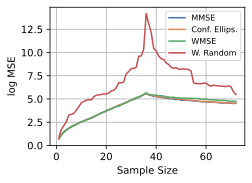
\includegraphics[width=\columnwidth]{plots/LS_MSE_real/fmri_subsample_500_367_bandwidth_36_SNRdbs_-10.0_samps_72_fb_blsig_MSE_LS.png}}
    \caption{Full-band noise, SNR = $10^{-1}$}
    \label{r1fmri_MSE_subfiga}
    \end{subfigure}\hfill
    \begin{subfigure}{0.3\columnwidth}
    \resizebox{\width}{0.62\columnwidth}{
    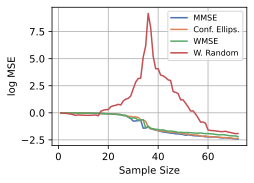
\includegraphics[width=\columnwidth]{plots/LS_MSE_real/fmri_subsample_500_367_bandwidth_36_SNRdbs_20.0_samps_72_fb_blsig_MSE_LS.png}}
    \caption{Full-band noise, SNR = $10^{2}$}%
    \label{r1fmri_MSE_subfigb___}%
    \end{subfigure}\hfill%
    \begin{subfigure}{0.3\columnwidth}
    \resizebox{\width}{0.62\columnwidth}{
    \includegraphics[width=\columnwidth]{plots/LS_MSE_real/fmri_subsample_500_367_bandwidth_36_SNRdbs_100.0_samps_72_fb_blsig_MSE_LS.png}}
    \caption{Full-band noise, SNR = $10^{10}$}%
    \label{r1fmri_MSE_subfigc}%
    \end{subfigure}%
    \hfill
    \iffalse
    \begin{subfigure}{0.3\columnwidth}
    \resizebox{\width}{0.62\columnwidth}{
    \includegraphics[width=\columnwidth]{plots/LS_MSE_real/fmri_subsample_500_367_bandwidth_36_SNRdbs_-10.0_samps_72_bl_blsig_MSE_LS.png}}
    \caption{Bandlimited noise, SNR = $10^{-1}$}
    \label{r1fmri_bandlimited_MSE_subfiga}
    \end{subfigure}\hfill
    \begin{subfigure}{0.3\columnwidth}
    \resizebox{\width}{0.62\columnwidth}{
    \includegraphics[width=\columnwidth]{plots/LS_MSE_real/fmri_subsample_500_367_bandwidth_36_SNRdbs_0.0_samps_72_bl_blsig_MSE_LS.png}}
    \caption{Bandlimited noise, SNR = $1$}%
    \label{r1bandlimited_MSE_subfigb}%
    \end{subfigure}\hfill%
    \begin{subfigure}{0.3\columnwidth}
    \resizebox{\width}{0.62\columnwidth}{
    \includegraphics[width=\columnwidth]{plots/LS_MSE_real/fmri_subsample_500_367_bandwidth_36_SNRdbs_100.0_samps_72_bl_blsig_MSE_LS.png}}
    \caption{Bandlimited noise, SNR = $10^{10}$}%
    \label{r1bandlimited_MSE_subfigc}%
    \end{subfigure}%
    \fi
    \caption{Average MSE under LS on the FMRI Graph (\#vertices=500, bandwidth = 50) }
\label{r1LS_fmri_MSE_fig}
\end{figure*}

\begin{figure*}[h!]%
    \centering
    \begin{subfigure}{0.3\columnwidth}
    \resizebox{\width}{0.62\columnwidth}{
    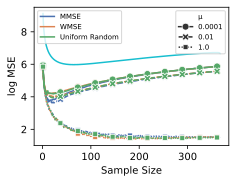
\includegraphics[width=\columnwidth]{plots/GLR_MSE_real/fmri_subsample_500_367_bandwidth_36_SNRdbs_-10.0_samps_367_mus_0.0001_0.01_1_full_band_MSE_GLR.png}}
    \caption{Full-band noise, SNR = $10^{-1}$}
    \label{r1GLR_MSE_subfiga}
    \end{subfigure}\hfill
    \begin{subfigure}{0.3\columnwidth}
    \resizebox{\width}{0.62\columnwidth}{
    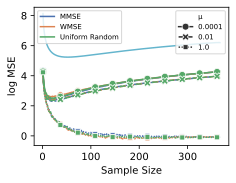
\includegraphics[width=\columnwidth]{plots/GLR_MSE_real/fmri_subsample_500_367_bandwidth_36_SNRdbs_-3.010299956639812_samps_367_mus_0.0001_0.01_1_full_band_MSE_GLR.png}}
    \caption{Full-band noise, SNR = $\frac{1}{2}$}%
    \label{r1GLR_MSE_subfigb}%
    \end{subfigure}\hfill%
    \begin{subfigure}{0.3\columnwidth}
    \resizebox{\width}{0.62\columnwidth}{
    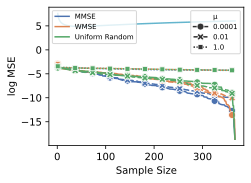
\includegraphics[width=\columnwidth]{plots/GLR_MSE_real/fmri_subsample_500_367_bandwidth_36_SNRdbs_100.0_samps_367_mus_0.0001_0.01_1_full_band_MSE_GLR.png}}
    \caption{Full-band noise, SNR = $10^{10}$}%
    \label{r1GLR_MSE_subfigc}%
    \end{subfigure}%
    
    \caption{Average MSE under GLR on FMRI Graph (line without markers is an upper bound)}
\label{r1GLR_fmri_MSE_fig}
%\label{bandlimited_GLR_ER_MSE_fig}
\end{figure*}





\begin{figure*}[h!]%
    \centering
    \begin{subfigure}{0.3\columnwidth}
    \resizebox{\width}{0.62\columnwidth}{
    \includegraphics[width=\columnwidth]{plots/LS_MSE_real/weather_45_bandwidth_8_SNRdbs_-10.0_samps_16_fb_blsig_MSE_LS.png}}
    \caption{Full-band noise, SNR = $10^{-1}$}
    \label{r1fmri_MSE_subfiga}
    \end{subfigure}\hfill
    \begin{subfigure}{0.3\columnwidth}
    \resizebox{\width}{0.62\columnwidth}{
    \includegraphics[width=\columnwidth]{plots/LS_MSE_real/weather_45_bandwidth_8_SNRdbs_20.0_samps_16_fb_blsig_MSE_LS.png}}
    \caption{Full-band noise, SNR = $10^{2}$}%
    \label{r1fmri_MSE_subfigb}%
    \end{subfigure}\hfill%
    \begin{subfigure}{0.3\columnwidth}
    \resizebox{\width}{0.62\columnwidth}{
    \includegraphics[width=\columnwidth]{plots/LS_MSE_real/weather_45_bandwidth_8_SNRdbs_100.0_samps_16_fb_blsig_MSE_LS.png}}
    \caption{Full-band noise, SNR = $10^{10}$}%
    \label{r1fmri_MSE_subfigc}%
    \end{subfigure}%
    \hfill
    \iffalse
    \begin{subfigure}{0.3\columnwidth}
    \resizebox{\width}{0.62\columnwidth}{
    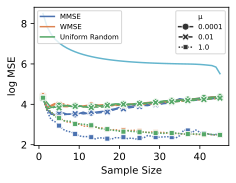
\includegraphics[width=\columnwidth]{plots/GLR_MSE_real/weather_45_bandwidth_8_SNRdbs_-10.0_samps_45_mus_0.0001_0.01_1_full_band_MSE_GLR.png}}
    \caption{Bandlimited noise, SNR = $10^{-1}$}
    \label{r1fmri_bandlimited_MSE_subfiga}
    \end{subfigure}\hfill
    \begin{subfigure}{0.3\columnwidth}
    \resizebox{\width}{0.62\columnwidth}{
    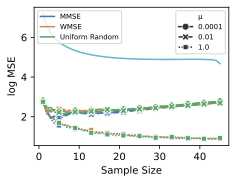
\includegraphics[width=\columnwidth]{plots/GLR_MSE_real/weather_45_bandwidth_8_SNRdbs_-3.010299956639812_samps_45_mus_0.0001_0.01_1_full_band_MSE_GLR.png}}
    \caption{Bandlimited noise, SNR = $1$}%
    \label{r1bandlimited_MSE_subfigb}%
    \end{subfigure}\hfill%
    \begin{subfigure}{0.3\columnwidth}
    \resizebox{\width}{0.62\columnwidth}{
    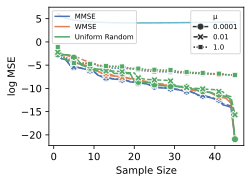
\includegraphics[width=\columnwidth]{plots/GLR_MSE_real/weather_45_bandwidth_8_SNRdbs_100.0_samps_45_mus_0.0001_0.01_1_full_band_MSE_GLR.png}}
    \caption{Bandlimited noise, SNR = $10^{10}$}%
    \label{r1bandlimited_MSE_subfigc}%
    \end{subfigure}%
    \fi
    \caption{Average MSE under LS on the Weather Graph (\#vertices=45, bandwidth = 8) }
\label{r1LS_weather_MSE_fig}
\end{figure*}

\begin{figure}[h!]%
    \centering
    \begin{subfigure}{0.3\columnwidth}
    \resizebox{\width}{0.62\columnwidth}{
    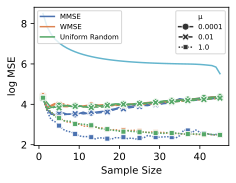
\includegraphics[width=\columnwidth]{plots/GLR_MSE_real/weather_45_bandwidth_8_SNRdbs_-10.0_samps_45_mus_0.0001_0.01_1_full_band_MSE_GLR.png}}
    \caption{Full-band noise, SNR = $10^{-1}$}
    \label{r1GLR_MSE_subfiga}
    \end{subfigure}\hfill
    \begin{subfigure}{0.3\columnwidth}
    \resizebox{\width}{0.62\columnwidth}{
    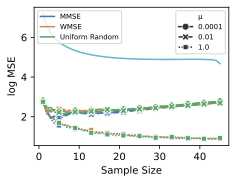
\includegraphics[width=\columnwidth]{plots/GLR_MSE_real/weather_45_bandwidth_8_SNRdbs_-3.010299956639812_samps_45_mus_0.0001_0.01_1_full_band_MSE_GLR.png}}
    \caption{Full-band noise, SNR = $\frac{1}{2}$}%
    \label{r1GLR_MSE_subfigb}%
    \end{subfigure}\hfill%
    \begin{subfigure}{0.3\columnwidth}
    \resizebox{\width}{0.62\columnwidth}{
    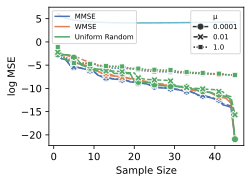
\includegraphics[width=\columnwidth]{plots/GLR_MSE_real/weather_45_bandwidth_8_SNRdbs_100.0_samps_45_mus_0.0001_0.01_1_full_band_MSE_GLR.png}}
    \caption{Full-band noise, SNR = $10^{10}$}%
    \label{r1GLR_MSE_subfigc}%
    \end{subfigure}%
    
    \caption{Average MSE under GLR on Weather Graph (line without markers is an upper bound)}
\label{r1GLR_weather_MSE_fig}
%\label{bandlimited_GLR_ER_MSE_fig}
\end{figure}

\begin{figure}[h!]%
    \centering
    \begin{subfigure}{0.4\columnwidth}
    \resizebox{\width}{0.62\columnwidth}{
    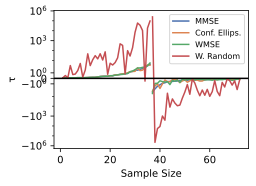
\includegraphics[width=\columnwidth]{plots/LS_threshold_real/fmri_subsample_500_367_bandwidth_36_thresholds_LS.png}}
    \caption{FMRI}
    \label{r1tau_FMRI_LS}
    \end{subfigure}\hfill
    \begin{subfigure}{0.4\columnwidth}
    \resizebox{\width}{0.62\columnwidth}{
    \includegraphics[width=\columnwidth]{plots/LS_threshold_real/weather_45_bandwidth_8_thresholds_LS.png}}
    \caption{Weather}
    \label{r1GLR_MSE_subfigb}%
    \end{subfigure}
    
    \caption{$\tau(\set{S},v)$ under LS reconstruction and full-band noise on different graphs }
\label{r1fig:LS_tau_real}
\end{figure}

\begin{figure}[h!]%
    \centering
    \begin{subfigure}{0.4\columnwidth}
    \resizebox{\width}{0.62\columnwidth}{
    \includegraphics[width=\columnwidth]{plots/GLR_threshold_real/fmri_subsample_500_GLR_threshold_fb.png}}
    \caption{FMRI}
    \label{r1tau_FMRI_GLR}
    \end{subfigure}\hfill
    \begin{subfigure}{0.4\columnwidth}
    \resizebox{\width}{0.62\columnwidth}{
    \includegraphics[width=\columnwidth]{plots/GLR_threshold_real/weather_GLR_threshold_fb.png}}
    \caption{Weather}
    \label{r1GLR_MSE_subfigb}%
    \end{subfigure}
    \caption{$\tau(\set{N},\set{S}^{c})$ under GLR reconstruction and full-band noise on different graphs }
\label{r1fig:GLR_tau_real}
%\label{bandlimited_GLR_ER_MSE_fig}
\end{figure}


\newpage
\section*{Responses to Reviewer \#2}
\textbf{Comment}
\begin{quote}
This paper is about sampling and reconstruction of signals on graphs. The main contribution is a detailed theoretical analysis, with a corresponding numerical validation, of the relationship between the sizes of the bandlimited subspace, sampling set, and signal to noise ration (SNR). The main finding is that the MSE is non monotonic with the size of the sampling set, and that in some low SNR scenarios reducing the size of the sampling set might be beneficial.

While this is a generally well written paper with theoretically sound results, I have a major issues with the narrow scope, presentation and usefulness of the results.
\end{quote}

\textbf{Response}
\begin{quote}
We thank the reviewer for recognising the soundness of our results. We address the concerns regarding scope, presentation, and application of our results in detail as follows.
\end{quote}

\textbf{Comment}
\begin{quote}
1. The signal model is very specific and unusual. They consider k-bandlimited signals with covariance matrix equal to a projector matrix of rank K. This projector matrix corresponds to the k-dimensional bandlimited subspace. While this is indeed a bandlimited model, this specific choice is unusual and not common in the literature. It feels very artificial and only chosen due to mathematical tractability, but it is not well justified.  
\end{quote}

\textbf{Response}
\begin{quote}
Thank you for your feedback, we agree this is an important point and address it from the following three perspectives. First of all, we believe that the $k$-bandlimitedness is a common assumption in the graph signal processing literature \cite{wang2018optimal, wang2019low,bai2020fast, puy2018random, tremblay2017determinantal}, as it corresponds to a common smoothness model for the signal.

% While choosing $k$-bandlimited signals as a signal model is common  , we agree than choosing this particular signal model for theory is not usual. We both justify it and show that the assumption is not essential to our argument.

Second, for a signal $\vect{x}$ that is almost surely bandlimited, we can show that if the covariance exists and is finite, i.e. $\expect{\sqnormvec{\vect{x}}} < \infty$, then the covariance $\matr{\Sigma}$ must have the property that $\projbl\matr{\Sigma}\projbl = \matr{\Sigma}$ (see a proof below). Therefore, in a sense, our choice of $\matr{\Sigma} = \projbl$ is the simplest possible choice of covariance for a signal model. An alternative way to look at this is, if we low-pass filter a random full-band Gaussian signal by only keeping its first $k$ graph Fourier coefficients, it will have a covariance that corresponds to our choice.
% especially as in this revision we no longer require our signal model to be Gaussian, just have this specific covariance and be zero-mean (see Section II-C).
\begin{proof}
 As $\vect{x}$ is bandlimited a.s., $ \projbl\vect{x} = \vect{x} \,  a.s.$. Therefore 
 \begin{align}
 \vect{\mu} &= \expect{\vect{x}} = \expect{\projbl\vect{x}} = \projbl\expect{\vect{x}} = \projbl\vect{\mu} \\
 \expect{\vect{x}\vect{x}^{T}} &= \expect{\projbl\vect{x}\vect{x}^{T}\projbl}
 = \projbl \expect{\vect{x}\vect{x}^{T}}\projbl 
 \end{align}
so
 \begin{align}
 \matr{\Sigma} &= \expect{\vect{x}\vect{x}^{T}} - \vect{\mu}\vect{\mu}^{T} = \projbl\expect{\vect{x}\vect{x}^{T}}\projbl - \projbl\vect{\mu}\vect{\mu}^{T}\projbl \\&= \projbl\matr{\Sigma}\projbl
 \end{align}
\end{proof}

Third, we present a new proposition (called Proposition 1) in the revised version of the paper showing that our general approach does not depend on a specific signal model, but just requiring the covariance matrix being finite, and thus every theorem we have has an equivalent under \emph{any} finite-variance signal model. This is because our results are fundamentally about increasing noise sensitivity. Note that despite our approach being applicable to any signal, our results which compute the SNR threshold $\tau$ -- the answer to the question of how high the noise needs to be for these phenomena to emerge -- are indeed dependent on the signal model we choose.


More specifically, our results on the shape of the MSE at high noise levels as sample size varies (illustrated in our experiments in Figs. 4 \& 5) are not signal model dependent: 
\begin{itemize}
    \item For LS, on any graph, under any signal model and noise with Covariance $\matr{I}_{N}$, if the sample selection scheme is noiseless-optimal for $k$-bandlimited signals, then at a high enough noise the reconstruction error will be a $\Lambda$-shaped curve as sample size varies. (Section III-D, Remark 5)
    \item For LS, on any graph, under any signal model and noise with Covariance $\projbl$, then at a high enough noise level reconstruction error is increasing with sample size. (Appendix A, Corollary 3.2)
    \item For GLR, for any graph that meets constraint (41) in Proposition 3, under any signal model and noise with Covariance $\matr{I}_{N}$, at high enough noise, samples of size $\lceil\sqrt{N}\rceil$ are better than $\set{N}$. (Section III-F, Proposition 3; illustrated in Fig. 1)
    \item For GLR, for any graph that meets constraint (54) in Theorem 4, under any signal model and noise with Covariance $\projbl$, at high enough noise, samples of size $m_{opt\_bl}$ are better than $\set{N}$. (Section III-G, Theorem 4)
\end{itemize}

Finally, it is natural to ask if being noiseless-optimal for $k$-bandlimited signals is a constraint that makes sense if the signal model is not $k$-bandlimited; we note that:
\begin{itemize}
    \item Any sample scheme will always pick $k$ samples which increase noise sensitivity (Proposition 2) -- this result does not depend on sample scheme and signal model, only that we are using LS reconstruction projecting down into $k$-bandlimited signals for the graph.
    \item To avoid `noiseless-optimality', one must actively choose nodes which add absolutely no information about a clean underlying $k$-bandlimited signal -- this is a strong restriction for a sample selection scheme, and a fundamentally strange one to use in concert with LS reconstruction.
\end{itemize}

\iffalse
In light of this, we have added Proposition 1, which states that our approach doesn't depend on the signal model at all, just on the covariance matrix being finite, and thus every theorem we have has an equivalent under \emph{any} finite-variance signal model. This is because our results are fundamentally about increasing noise sensitivity. 


Specifically, our results on the shape of the MSE at high noise levels as sample size varies are not signal model dependent. 

For GLR, for any graph that meets our constraints, under any signal model and our noise model, at high enough noise, samples of size $\lceil\sqrt{N}\rceil$ are better than $\set{N}$.

For LS, on any graph, under any signal model and our noise model, if the sample selection scheme is noiseless-optimal for $k$-bandlimited noise, then at a high enough noise the reconstruction error will be a $\Lambda$-shaped curve with a peak at $k$ as sample size varies.


However, our computations of $\tau$ -- the answer to the question of how high the noise needs to be for these phenomena to emerge -- is indeed dependent on the signal model we choose.

It is natural to ask if being noiseless-optimal for $k$-bandlimited signals is a constraint that makes sense if the signal model is not $k$-bandlimited; we note that:
\begin{itemize}
    \item Any sample scheme will always pick $k$ samples which increase noise sensitivity, regardless of the signal model (Proposition 2 -- this comes from LS projecting into a $k$-dimensional space)
    \item To avoid 'noiseless-optimality', one must actively choose nodes which add absolutely no information about a clean underlying $k$-bandlimited signal -- this is a strong restriction for a sample selection scheme, and a fundamentally strange one to use in concert with LS reconstruction.
\end{itemize}
\fi
\end{quote}


\textbf{Comment}
\begin{quote}
2. Interpolation methods: The authors choose two linear interpolation methods, which are evaluated using MSE.  The interpolation methods to be studied in this paper (table I) are linear. It is known that for Gaussians signals with Gaussian noise (as in this paper’s model), the best reconstruction in the MSE sense to reconstruct x from y is linear and known in closed form (conditional expectation).  Since the error analysis is done using the MSE metric (last equation in Section II), I am surprised the analysis of this paper does not incorporate such a benchmark, thus the analysis is missing a major piece of related work.
\end{quote}

\textbf{Response}
\begin{quote}
Thank you for raising this point. We originally referred to this as `Optimal Bayesian Reconstruction' in Introduction, and it is known that increasing sample size must decrease MSE in this case \cite{chamon2017greedy}. However, this setting is different from the one we focus on in this paper. 
% Thus, we believe benchmarks involving this would not be additive.
We have now mentioned this in Section II-C alongside the other reconstruction/interpolation methods, and explicitly stated that we do not study methods where the reconstruction matrix is dependent on $\sigma$, as noise-aware reconstruction is not the focus of this paper (we have added a Remark in Section II.C to clarify this).

In the revised paper, we have also broadened the scope of the analysis so that the noise model no longer requires to be Gaussian, and clarified that our general approach actually does not depend on a specific signal model (as discussed in the response above). As a consequence, our analysis goes beyond the Gaussian settings.
\end{quote}

\textbf{Comment}
\begin{quote}
3. Beyond Gaussian signals and synthetic data. While it is interesting to understand the relationships between SNR and sampling set size, the paper does not offer any application or use case of this work. As is, the paper is just a detailed theoretical analysis of a signal/noise model, using two carefully chosen reconstruction methods, that depend on the signal model, with all experiments performed on simulated data using random Gaussian signals,  reconstructions algorithms that know the statistics of the data, and synthetic random graphs.  The paper shows no evidence that these results can be useful in any non-synthetic scenario.
I encourage the authors to consider either experiments with real data/graphs, and/or applications to sampling set selection,  for example you could test the effectiveness of early stop in greedy sampling algorithms in low SNR regimes, as suggested in the conclusions.
\end{quote}

\textbf{Response}
\begin{quote}
Thank you for raising this important point. 

First of all, as discussed in the responses above, we have broadened the scope of our analysis so hopefully it has a more general appeal to the community.

Second, in light of your comments, we have now adopted two real-world datasets, one based on FMRI data and one based on weather data. These are two real world datasets with real world signals. We have subsampled real world graphs (following \cite{zhi2023gaussian}), bandlimited the signals and added noise to match the setting in our paper. Details are in the Experiments section (Section IV) of the revised paper. We have copied the resultant figures into this document; they are Figs. \ref{LS_fmri_MSE_fig}-\ref{fig:GLR_tau_real}. 
Figs. \ref{LS_fmri_MSE_fig}-\ref{GLR_weather_MSE_fig} show that decreasing sample size can decrease MSE at sufficiently high noise levels even on real graphs and with signals sourced from real world data. This is consistent with Proposition 1 in the revised paper.

Third, we demonstrate the practical utility of our results as follows. For the different reconstruction methods, our theoretical results suggest the following algorithms for improving a sampling set by reduction, for LS and GLR reconstruction respectively. More specifically:

    For LS reconstruction, if we have chosen $k$ or fewer nodes by some noiseless-optimal scheme, we can calculate $\tau(\set{S},v)$ for each element of $\set{S}$, remove $v$ if $\text{SNR} < \tau(\set{S},v)$, and repeat until we can no longer find a node $v$ in our remaining set $\set{S}_{rem}$ where $\text{SNR} < \tau(\set{S}_{rem},v)$.

    If we have sampled more than $k$ nodes by a noiseless optimal scheme, we can still attempt this (and if removing $v$ is rank reducing and the noise is high enough this will still improve reconstruction performance on average, by the proof of Corollary 1.1). However, there is no guarantee that we can do so by removing any single node in this case, at any noise level.

    In the GLR case with fixed $\mu$, our theorem suggests the following, when we think our signal model applies. Given the graph structure, before observing any nodes:
\begin{enumerate}
    \item Check whether  condition (31) in Theorem 3 applies (this only depend on graph structure)
    \item If they do, compute $\tau_{GLR}$
    \item If we believe that $\text{SNR} < \tau_{GLR}$ holds, then sample $\lceil\sqrt{N}\rceil$ nodes at random and reconstruct from those nodes. We can choose the nodes at random as our theorem holds true for all $\set{S}$ of size $\lceil\sqrt{N}\rceil$.
\end{enumerate}


We now justify this method would work via examination of the experiments.
While we know in these cases that there is a threshold $\tau > 0$ (from our new Proposition 1), the calculation of $\tau$ depends on our assumptions around the signal model. Even though we cannot know for sure what the real world signal model is, we have assumed our signal model has covariance $\projbl$ in order to calculate $\tau$. Despite this, the real-world results are broadly consistent with the synthetic results -- if we look at SNR=$10^{2}$, for Fig \ref{tau_FMRI_LS_} we see the red line (Weighted Random sampling) is broadly above $10^2$ and the other lines (MMSE, WMSE and Confidence Ellipse Sampling) are below $10^2$. This is consistent with Fig \ref{fmri_MSE_subfigb__} where at SNR=$10^{2}$ -- we see that Weighted Random sampling has a $\Lambda$-shaped error and the other sampling methods have error decreasing as sample size increases. This demonstrates that the above algorithm, which are a consequence of our results, would improve reconstruction accuracy on real world data.


%These demonstrate the applicability of our theorems to real-world, non-synthetic graphs.

%We also provide plots of $\tau$ for these graphs under LS and GLR (Figs. \ref{fig:LS_tau_real} and \ref{fig:GLR_tau_real}). This allows for the following sampling algorithms for LS and GLR:


\begin{figure*}[h!]%
    \centering
    \begin{subfigure}{0.3\columnwidth}
    \resizebox{\width}{0.62\columnwidth}{
    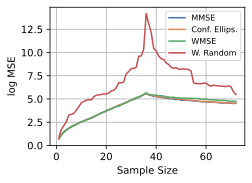
\includegraphics[width=\columnwidth]{plots/LS_MSE_real/fmri_subsample_500_367_bandwidth_36_SNRdbs_-10.0_samps_72_fb_blsig_MSE_LS.png}}
    \caption{Full-band noise, SNR = $10^{-1}$}
    \label{fmri_MSE_subfiga}
    \end{subfigure}\hfill
    \begin{subfigure}{0.3\columnwidth}
    \resizebox{\width}{0.62\columnwidth}{
    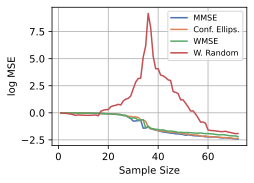
\includegraphics[width=\columnwidth]{plots/LS_MSE_real/fmri_subsample_500_367_bandwidth_36_SNRdbs_20.0_samps_72_fb_blsig_MSE_LS.png}}
    \caption{Full-band noise, SNR = $10^{2}$}%
    \label{fmri_MSE_subfigb__}%
    \end{subfigure}\hfill%
    \begin{subfigure}{0.3\columnwidth}
    \resizebox{\width}{0.62\columnwidth}{
    \includegraphics[width=\columnwidth]{plots/LS_MSE_real/fmri_subsample_500_367_bandwidth_36_SNRdbs_100.0_samps_72_fb_blsig_MSE_LS.png}}
    \caption{Full-band noise, SNR = $10^{10}$}%
    \label{fmri_MSE_subfigc}%
    \end{subfigure}%
    \hfill
    \iffalse
    \begin{subfigure}{0.3\columnwidth}
    \resizebox{\width}{0.62\columnwidth}{
    \includegraphics[width=\columnwidth]{plots/LS_MSE_real/fmri_subsample_500_367_bandwidth_36_SNRdbs_-10.0_samps_72_bl_blsig_MSE_LS.png}}
    \caption{Bandlimited noise, SNR = $10^{-1}$}
    \label{fmri_bandlimited_MSE_subfiga}
    \end{subfigure}\hfill
    \begin{subfigure}{0.3\columnwidth}
    \resizebox{\width}{0.62\columnwidth}{
    \includegraphics[width=\columnwidth]{plots/LS_MSE_real/fmri_subsample_500_367_bandwidth_36_SNRdbs_0.0_samps_72_bl_blsig_MSE_LS.png}}
    \caption{Bandlimited noise, SNR = $1$}%
    \label{bandlimited_MSE_subfigb}%
    \end{subfigure}\hfill%
    \begin{subfigure}{0.3\columnwidth}
    \resizebox{\width}{0.62\columnwidth}{
    \includegraphics[width=\columnwidth]{plots/LS_MSE_real/fmri_subsample_500_367_bandwidth_36_SNRdbs_100.0_samps_72_bl_blsig_MSE_LS.png}}
    \caption{Bandlimited noise, SNR = $10^{10}$}%
    \label{bandlimited_MSE_subfigc}%
    \end{subfigure}%
    \fi
    \caption{Average MSE under LS on the FMRI Graph (\#vertices=500, bandwidth = 50) }
\label{LS_fmri_MSE_fig}
\end{figure*}

\begin{figure*}[h!]%
    \centering
    \begin{subfigure}{0.3\columnwidth}
    \resizebox{\width}{0.62\columnwidth}{
    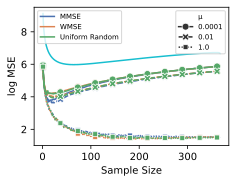
\includegraphics[width=\columnwidth]{plots/GLR_MSE_real/fmri_subsample_500_367_bandwidth_36_SNRdbs_-10.0_samps_367_mus_0.0001_0.01_1_full_band_MSE_GLR.png}}
    \caption{Full-band noise, SNR = $10^{-1}$}
    \label{GLR_MSE_subfiga}
    \end{subfigure}\hfill
    \begin{subfigure}{0.3\columnwidth}
    \resizebox{\width}{0.62\columnwidth}{
    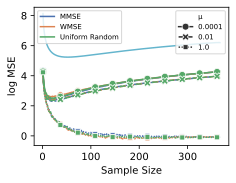
\includegraphics[width=\columnwidth]{plots/GLR_MSE_real/fmri_subsample_500_367_bandwidth_36_SNRdbs_-3.010299956639812_samps_367_mus_0.0001_0.01_1_full_band_MSE_GLR.png}}
    \caption{Full-band noise, SNR = $\frac{1}{2}$}%
    \label{GLR_MSE_subfigb}%
    \end{subfigure}\hfill%
    \begin{subfigure}{0.3\columnwidth}
    \resizebox{\width}{0.62\columnwidth}{
    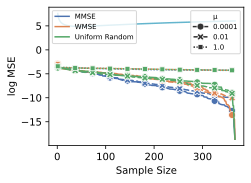
\includegraphics[width=\columnwidth]{plots/GLR_MSE_real/fmri_subsample_500_367_bandwidth_36_SNRdbs_100.0_samps_367_mus_0.0001_0.01_1_full_band_MSE_GLR.png}}
    \caption{Full-band noise, SNR = $10^{10}$}%
    \label{GLR_MSE_subfigc}%
    \end{subfigure}%
    
    \iffalse
    \hfill
    \begin{subfigure}{0.3\columnwidth}
    \resizebox{\width}{0.62\columnwidth}{
    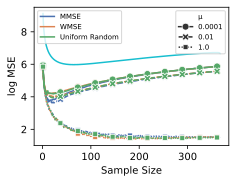
\includegraphics[width=\columnwidth]{plots/GLR_MSE_real/fmri_subsample_500_367_bandwidth_36_SNRdbs_-10.0_samps_367_mus_0.0001_0.01_1_full_band_MSE_GLR.sv}}
    \caption{Bandlimited noise, SNR = $10^{-2}$}
    \label{bandlimited_GLR_MSE_subfiga}
    \end{subfigure}\hfill
    \begin{subfigure}{0.3\columnwidth}
    \resizebox{\width}{0.62\columnwidth}{
    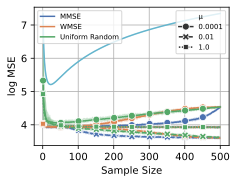
\includegraphics[width=\columnwidth]{plots/GLR_MSE/ER_0pt8_500_bandwidth_50_SNRdbs_-3.01_samps_500_mus_0.0001_0.01_1_bl_noise.png}}
    \caption{Bandlimited noise, SNR = $\frac{1}{2}$}%
    \label{bandlimited_GLR_MSE_subfigb}%
    \end{subfigure}\hfill%
    \begin{subfigure}{0.3\columnwidth}
    \resizebox{\width}{0.62\columnwidth}{
    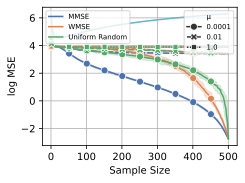
\includegraphics[width=\columnwidth]{plots/GLR_MSE/ER_0pt8_500_bandwidth_50_SNRdbs_100.0_samps_500_mus_0.0001_0.01_1_bl_noise.png}}
    \caption{Bandlimited noise, SNR = $10^{10}$}%
    \label{bandlimited_GLR_MSE_subfigc}%
    \end{subfigure}%
    \fi
    \caption{Average MSE under GLR on FMRI Graph (line without markers is an upper bound)}
\label{GLR_fmri_MSE_fig}
%\label{bandlimited_GLR_ER_MSE_fig}
\end{figure*}





\begin{figure*}[h!]%
    \centering
    \begin{subfigure}{0.3\columnwidth}
    \resizebox{\width}{0.62\columnwidth}{
    \includegraphics[width=\columnwidth]{plots/LS_MSE_real/weather_45_bandwidth_8_SNRdbs_-10.0_samps_16_fb_blsig_MSE_LS.png}}
    \caption{Full-band noise, SNR = $10^{-1}$}
    \label{fmri_MSE_subfiga}
    \end{subfigure}\hfill
    \begin{subfigure}{0.3\columnwidth}
    \resizebox{\width}{0.62\columnwidth}{
    \includegraphics[width=\columnwidth]{plots/LS_MSE_real/weather_45_bandwidth_8_SNRdbs_20.0_samps_16_fb_blsig_MSE_LS.png}}
    \caption{Full-band noise, SNR = $10^{2}$}%
    \label{fmri_MSE_subfigb}%
    \end{subfigure}\hfill%
    \begin{subfigure}{0.3\columnwidth}
    \resizebox{\width}{0.62\columnwidth}{
    \includegraphics[width=\columnwidth]{plots/LS_MSE_real/weather_45_bandwidth_8_SNRdbs_100.0_samps_16_fb_blsig_MSE_LS.png}}
    \caption{Full-band noise, SNR = $10^{10}$}%
    \label{fmri_MSE_subfigc}%
    \end{subfigure}%
    \hfill
    \iffalse
    \begin{subfigure}{0.3\columnwidth}
    \resizebox{\width}{0.62\columnwidth}{
    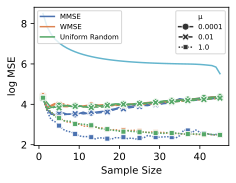
\includegraphics[width=\columnwidth]{plots/GLR_MSE_real/weather_45_bandwidth_8_SNRdbs_-10.0_samps_45_mus_0.0001_0.01_1_full_band_MSE_GLR.png}}
    \caption{Bandlimited noise, SNR = $10^{-1}$}
    \label{fmri_bandlimited_MSE_subfiga}
    \end{subfigure}\hfill
    \begin{subfigure}{0.3\columnwidth}
    \resizebox{\width}{0.62\columnwidth}{
    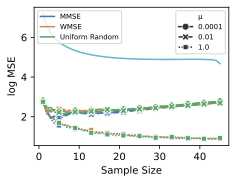
\includegraphics[width=\columnwidth]{plots/GLR_MSE_real/weather_45_bandwidth_8_SNRdbs_-3.010299956639812_samps_45_mus_0.0001_0.01_1_full_band_MSE_GLR.png}}
    \caption{Bandlimited noise, SNR = $1$}%
    \label{bandlimited_MSE_subfigb}%
    \end{subfigure}\hfill%
    \begin{subfigure}{0.3\columnwidth}
    \resizebox{\width}{0.62\columnwidth}{
    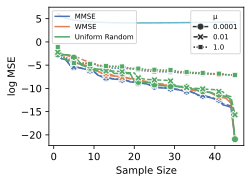
\includegraphics[width=\columnwidth]{plots/GLR_MSE_real/weather_45_bandwidth_8_SNRdbs_100.0_samps_45_mus_0.0001_0.01_1_full_band_MSE_GLR.png}}
    \caption{Bandlimited noise, SNR = $10^{10}$}%
    \label{bandlimited_MSE_subfigc}%
    \end{subfigure}%
    \fi
    \caption{Average MSE under LS on the Weather Graph (\#vertices=45, bandwidth = 8) }
\label{LS_weather_MSE_fig}
\end{figure*}

\begin{figure}[h!]%
    \centering
    \begin{subfigure}{0.3\columnwidth}
    \resizebox{\width}{0.62\columnwidth}{
    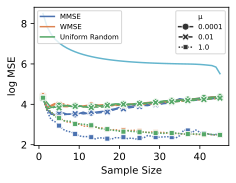
\includegraphics[width=\columnwidth]{plots/GLR_MSE_real/weather_45_bandwidth_8_SNRdbs_-10.0_samps_45_mus_0.0001_0.01_1_full_band_MSE_GLR.png}}
    \caption{Full-band noise, SNR = $10^{-1}$}
    \label{GLR_MSE_subfiga}
    \end{subfigure}\hfill
    \begin{subfigure}{0.3\columnwidth}
    \resizebox{\width}{0.62\columnwidth}{
    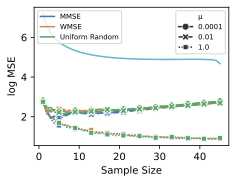
\includegraphics[width=\columnwidth]{plots/GLR_MSE_real/weather_45_bandwidth_8_SNRdbs_-3.010299956639812_samps_45_mus_0.0001_0.01_1_full_band_MSE_GLR.png}}
    \caption{Full-band noise, SNR = $\frac{1}{2}$}%
    \label{GLR_MSE_subfigb}%
    \end{subfigure}\hfill%
    \begin{subfigure}{0.3\columnwidth}
    \resizebox{\width}{0.62\columnwidth}{
    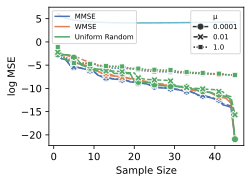
\includegraphics[width=\columnwidth]{plots/GLR_MSE_real/weather_45_bandwidth_8_SNRdbs_100.0_samps_45_mus_0.0001_0.01_1_full_band_MSE_GLR.png}}
    \caption{Full-band noise, SNR = $10^{10}$}%
    \label{GLR_MSE_subfigc}%
    \end{subfigure}%
    
    \iffalse
    \hfill
    \begin{subfigure}{0.3\columnwidth}
    \resizebox{\width}{0.62\columnwidth}{
    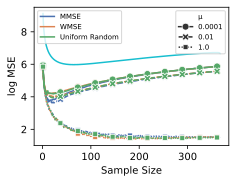
\includegraphics[width=\columnwidth]{plots/GLR_MSE_real/fmri_subsample_500_367_bandwidth_36_SNRdbs_-10.0_samps_367_mus_0.0001_0.01_1_full_band_MSE_GLR.sv}}
    \caption{Bandlimited noise, SNR = $10^{-2}$}
    \label{bandlimited_GLR_MSE_subfiga}
    \end{subfigure}\hfill
    \begin{subfigure}{0.3\columnwidth}
    \resizebox{\width}{0.62\columnwidth}{
    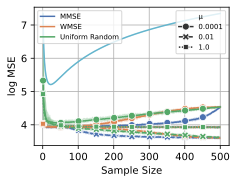
\includegraphics[width=\columnwidth]{plots/GLR_MSE/ER_0pt8_500_bandwidth_50_SNRdbs_-3.01_samps_500_mus_0.0001_0.01_1_bl_noise.png}}
    \caption{Bandlimited noise, SNR = $\frac{1}{2}$}%
    \label{bandlimited_GLR_MSE_subfigb}%
    \end{subfigure}\hfill%
    \begin{subfigure}{0.3\columnwidth}
    \resizebox{\width}{0.62\columnwidth}{
    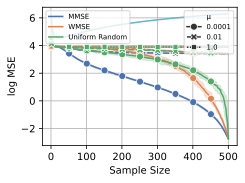
\includegraphics[width=\columnwidth]{plots/GLR_MSE/ER_0pt8_500_bandwidth_50_SNRdbs_100.0_samps_500_mus_0.0001_0.01_1_bl_noise.png}}
    \caption{Bandlimited noise, SNR = $10^{10}$}%
    \label{bandlimited_GLR_MSE_subfigc}%
    \end{subfigure}%
    \fi
    \caption{Average MSE under GLR on Weather Graph (line without markers is an upper bound)}
\label{GLR_weather_MSE_fig}
%\label{bandlimited_GLR_ER_MSE_fig}
\end{figure}

\begin{figure}[h!]%
    \centering
    \begin{subfigure}{0.4\columnwidth}
    \resizebox{\width}{0.62\columnwidth}{
    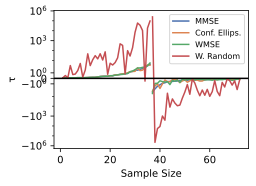
\includegraphics[width=\columnwidth]{plots/LS_threshold_real/fmri_subsample_500_367_bandwidth_36_thresholds_LS.png}}
    \caption{FMRI}
    \label{tau_FMRI_LS_}
    \end{subfigure}\hfill
    \begin{subfigure}{0.4\columnwidth}
    \resizebox{\width}{0.62\columnwidth}{
    \includegraphics[width=\columnwidth]{plots/LS_threshold_real/weather_45_bandwidth_8_thresholds_LS.png}}
    \caption{Weather}
    \label{GLR_MSE_subfigb}%
    \end{subfigure}
    
    \caption{$\tau(\set{S},v)$ under LS reconstruction and full-band noise on different graphs }
\label{fig:LS_tau_real}
\end{figure}

\begin{figure}[h!]%
    \centering
    \begin{subfigure}{0.4\columnwidth}
    \resizebox{\width}{0.62\columnwidth}{
    \includegraphics[width=\columnwidth]{plots/GLR_threshold_real/fmri_subsample_500_GLR_threshold_fb.png}}
    \caption{FMRI}
    \label{tau_FMRI_LS}
    \end{subfigure}\hfill
    \begin{subfigure}{0.4\columnwidth}
    \resizebox{\width}{0.62\columnwidth}{
    \includegraphics[width=\columnwidth]{plots/GLR_threshold_real/weather_GLR_threshold_fb.png}}
    \caption{Weather}
    \label{GLR_MSE_subfigb}%
    \end{subfigure}
    \caption{$\tau(\set{N},\set{S}^{c})$ under GLR reconstruction and full-band noise on different graphs }
\label{fig:GLR_tau_real}
%\label{bandlimited_GLR_ER_MSE_fig}
\end{figure}
\end{quote}

\clearpage
\textbf{Comment}
\begin{quote}
4. Organization of main results:  It is hard to connect the contributions (1,2 and 3) stated in the introduction to the main results. Section III is hard to follow. It is not clear what are the most important results, and what is the significance. I suggest spending more time on organizing section III, and emphasizing the most important results.
\end{quote}

\textbf{Response}
\begin{quote}
Thank you for the feedback. 
\iffalse
We have reworked Section III to be easier to follow. As presented in Introduction, our first three contributions are:
\begin{enumerate}
    \item A theoretical characterisation of how decreasing sample size may decrease MSE, not only under LS  but also under GLR, a regularised method. 
    \item Analysis of both LS and GLR under bandlimited noise to show non-monotonicity of the MSE is not caused by just the high frequency component of the noise.
    \item Asymptotic analysis, showing how the non-monotonicity of the MSE with sample size persists as $N \to \infty$.
\end{enumerate}

To make it clearer how these connect to the main results, we have added Table II in Section III-A, which we copy below. 
\fi
We have made multiple efforts in the revised paper to improve the presentation of main results:
\begin{itemize}
\item We have provided a general overview of the paper in Introduction, with clearly states which results are covered in which sections. 
\item %We have added a new Table III in Section III.A, which helps illustrates the structure of the theoretical results in Section III; 
In Section III-A which gives a proof overview and breaks our approach into four steps, we present a new Table III which shows how Sections III-D to III-G follow those four steps -- outlining which results correspond to which step. This should help readers understand how each of the stages of Section III-F and III-G (which has been moved to Appendix B in the revised paper) correspond to the steps taken in previous sections and the overall plan. It also highlights the major results. The added table is presented here:

\begin{table}[h]
\caption{Structure of Theoretical Results}
\centering
\begin{tabular}{|l|c|c|c|c|c|}
\hline
 & General &\multicolumn{2}{c|}{LS} & \multicolumn{2}{c|}{GLR} \\
\hline
{Noise} & Any & Full-band & Band-limited & Full-band & Band-limited \\
\hline
\emph{Simplification} & $\set{S} \supset \set{T}$ & \multicolumn{2}{c|}{$\set{S}$ vs $\set{S} \backslash \{v\}$} &  \multicolumn{2}{c|}{$\set{N}$ vs $\set{S}$}  \\
\hline
\emph{Characterisation} & Thm 1 & Corr 1,1 & Corr 3.2 & \multicolumn{2}{c|}{Corr 2.1}  \\
\hline
\emph{Existence} & & Thm 2 & Corr 3.3 & Thm 3 & Thm 4 \\
\hline
\emph{Asymptotics} & & Remark 8 & Remark 10 & Propn 4 & Propn 5 \\
\hline
\end{tabular}
\label{tbl:general_theory}
\end{table}

\iffalse
This table acts as an overall guide on how each section is structured, and connects the contributions to the results in the following way:
\begin{enumerate}
    \item The characterisation is in the 'characterisation' column (and the 'existence' column gives a specific characterisation, more directly showing circumstances when reducing sample size reduces MSE)
    \item We see the relevant results in the 'bandlimited' rows; they correspond to Sections III-E and III-G
    \item This is presented in the Asymptotics column.
\end{enumerate}
\fi

\item We have reorganised Section III to make it clearer and easier to follow. In particular, we have done a major revision of Section III.F to improve its clarity and interpretability. We have also decided to move detailed results on bandlimited settings to Appendix to simplify this section (we are however open to further comments and suggestions on this change).
\item We have added a new Table V, which aligns with the new Table III and provide a roadmap for reading the experimental results. We hope all these efforts help improve the exposition of the paper and makes it easier for the reader to follow.
\end{itemize}

We hope all these efforts help improve the exposition
of the main results and makes them easier for the reader to follow.

\end{quote}

\textbf{Comment}
\begin{quote}
Technical comment regarding equation (12) and (15).

The LS interpolator, as well as many other reconstruction algorithms, is sample consistent, that is, the reconstructed signal is equal to the original signal, when restricted to the sampling set.  For this paper, the LS reconstruction is unbiased on the sampling set S, and thus only the reconstructed signal in the complement of S will contribute to the error. This would imply that the variance and bias formulas from (12) can be simplified for this reconstruction, which may affect subsequent results such as (15), and others in section III. Please clarify.
\end{quote}

\textbf{Response}
\begin{quote}
Thank you for rising this point. First of all we note that GLR for $\mu>0$ is not sample consistent, so we focus our response on the LS reconstruction.

We first discuss the bias term in (12). We agree that under LS reconstruction we can simplify the bias term in (12), which is also represented in (15), under the case of LS reconstruction by using sample consistency. This is fundamental to the construction of Table IV in section III-C in the revised paper, and the explicit result simplifying (15) is Appendix G, Lemma 4. This is the reason that $\Delta_{1}(\set{S},v)$ only takes the values $0$ and $-1$.

We would like to point out that we did make use of the sample consistency in Lemma 4 even though this is somewhat opaque -- we use the 'weak inverse' property of the Moore-Penrose psuedoinverse, which we will now prove is equivalent to sample consistency, and show how it is core to Lemma 4 which drives Table IV which is the core of our LS analysis under full band noise.

\begin{proof}
We first disambiguate
\begin{itemize}
    \item The clean underlying signal: $\vect{x}$,
    \item The noise-corrupted observed signal observed at $\set{S}$: $\vectsub[S]{y}$,
    \item The reconstructed signal: $\hat{\vect{x}}$.
\end{itemize}
For mathematical convenience, we imagine $\vect{y}$ is the noise-corrupted observation of the signal on all nodes, and that $\vectsub[S]{y}$ is its restriction to $\set{S}$. This $\vect{y}$ is a merely useful mathematical fiction -- our proof holds even if we never observe all of the nodes. In the noiseless case, such a $\vect{y}$ would be $k$-bandlimited.

We discuss the noiseless case, where we agree that $\vectsub[S]{x} = \vectsub[S]{y} = \vectsub[S]{\hat{\vect{x}}}$ for LS. We do implicitly use this statement in the proof of Lemma 4. Writing $\vect{y} = \matrsubU{N}\vect{v}_{k}$ and so $\vectsub[S]{y} = \matrsubU{S}\vect{v}_{k}$, we have the following statements which are all equivalent:
\begin{align}
    &\forall \vect{y}\,  k\text{-bandlimited}, \quad \vectsub[S]{y} - \vectsub[S]{\hat{x}} = \vect{0} \quad\text{i.e. sample consistency}\\
    &\forall \vect{y}\,  k\text{-bandlimited}, \quad \vectsub[S]{y} - \matrsub[S,N]{I}\matr{R}_{\set{S}}\vectsub[S]{y} = \vect{0}\\
    &\forall \vect{v}_{k}\in\mathbb{R}^{k}, \quad \matrsubU{S}\vect{v}_{k} - \matrsub[S,N]{I}\matr{R}_{\set{S}}\matrsubU{S}\vect{v}_{k} = \vect{0} \\
    &\matrsubU{S} - \matrsub[S,N]{I}\matr{R}_{\set{S}}\matrsubU{S} = \vect{0}\\
    &\matrsubU{S} - \matrsubU{S}\left(\matrsubU{S}\right)^{\dagger}\matrsubU{S} = \vect{0} \\
    &\matrsubU{S} = \matrsubU{S}\left(\matrsubU{S}\right)^{\dagger}\matrsubU{S}  \label{eq:rev2_AAplusA}
\end{align}

As a consequence of (\ref{eq:rev2_AAplusA}), we have
\begin{equation}
    \left(\matrsubU{S}\right)^{\dagger}\matrsubU{S} = \left(\matrsubU{S}\right)^{\dagger}\matrsubU{S}\left(\matrsubU{S}\right)^{\dagger}\matrsubU{S} 
\end{equation}
Thus $\matr{\Pi} = \left(\matrsubU{S}\right)^{\dagger}\matrsubU{S}$ is idempotent, so its eigenvalues satisfy $\lambda_{i}^{2} = \lambda_{i}$. The reconstruction must only supply real values, so $\matr{\Pi}$ must be real, and it is symmetric. Therefore its eigenvalues are real and are 0 or 1.

Furthermore, by (\ref{eq:rev2_AAplusA}) $\matr{\Pi}$ leaves $\matrsubU{S}$ invariant so $\rank{\matr{\Pi}} \geq \rank{\matrsubU{S}}$ ; and as $\matr{\Pi}$ is of the form $\matrsubU{S}\matr{X}$, $\rank{\matr{\Pi}} \leq \rank{\matrsubU{S}}$; therefore  $\rank{\matr{\Pi}} = \rank{\matrsubU{S}}$. This with the previous statement that its eigenvalues are 0 or 1 gives that $\trace{\matr{\Pi}} = \rank{\matrsubU{S}}$.

We know the reconstruction then has to `fill in the rest of the values' in our bandlimited basis, which is of dimension $k$, giving
\begin{equation}
    \xi_{1}(\set{S}) = k - \rank{\matrsubU{S}},
\end{equation}
which, as shown above, intimately uses the sample consistency of recontruction. More details are provided in the proof of Lemma 4 in Appendix G.

\end{proof}

We then discuss the variance term in (12). 
Table IV uses this characterisation of error to characterise the increase or decrease in the variance term in (12). However, error in the variance term can come from the observed nodes, and thus it is difficult to simplify this term using sample consistency. We now see this by considering the noisy case. For example, imagine that the signal is $\vect{x} = 0$ and the noise is high frequency (e.g. $\vect{u}_{N}$, the highest frequency eigenvector). Then on observing all nodes and applying $\matr{R}_{N}$, the reconstructed signal will be $\hat{\vect{x}} = 0$. However, $\vectsub[N]{y} = \vect{u}_{N}$ which is not 0 everywhere. This is because least squares smooths high frequency signals on the observed nodes, and thus we cannot only look at the variance term error on $\set{S}^{C}$.
\end{quote}

\textbf{Comment}
\begin{quote}
Other minor comments
\begin{itemize}
\item A few equations in the paper do not have numbers, please add numbers to all of them.  I do not see a reason to not number all equations.
\item The formula from equation (12) should be available in a book, you may save some space by removing the derivation and adding a citation.
\item In the experiments be clearer as to which sampling algorithms were used, and please include references.
\end{itemize}
\end{quote}

\textbf{Response}
\begin{quote}
Thank you for pointing these out. We have:
\begin{itemize}
    \item added equation numbers to all equations
    \item moved the derivation of the bias-variance decomposition to the Appendix and also added a citation
    \item added citations corresponding to the sampling algorithms used in the experimental setup section (Section IV-A). We note that the sampling algorithms are further discussed in Section II-D.
\end{itemize}
\end{quote}

\newpage
\section*{Responses to Reviewer \#3}
\textbf{Comment}
\begin{quote}
    This paper studied a novel perspective on the sampling and recovery of graph signals with limited bandwidth. Specifically, the paper investigates scenarios where a reduction in the number of samples can paradoxically lead to improved recovery performance. This is an intriguing research point. In conclusion, they investigate conditions to support this phenomena for unbiased LS and biased GLR reconstruction where noise model is bandlimited or full-band.  It suggests for LS recovery that below a certain signal-to-noise ratio threshold and when the sampling number is less than the bandwidth, performance can be improved with fewer samples. For GLR, they focus on the simplification for comparing full / almost full observation with partial observations, which indicates fewer samples will have better performance compared to selecting all samples if SNR is less than some threshold.
\end{quote}

\textbf{Response}
\begin{quote}
We thank the reviewer for their positive evaluation of our paper.
\end{quote}

\textbf{Comment}
\begin{quote}
 However, my major concern about this paper is about its value to guide practical design of sampling and reconstruction methods of BL graph signals. Although pure theoretical study is very important, its close connection for algorithm development is also very important to me.  Therefore, before supporting its publication on TSP, the top journal in SP society, we still need the authors to solve my following concerns:
 \end{quote}
 
\textbf{Response}
\begin{quote}
We completely agree with the reviewer on this point and we address their concerns in detail as follows.
\end{quote}
 
\textbf{Comment}
\begin{quote}
(1)While the research focus is unique, I must voice my skepticism regarding the practical utility of the outcomes. It would be beneficial to delve deeper into the implications of these findings in real-world applications, a point which I hope the authors emphasize at the very beginning of the article. Why is the focus of this paper, to find condition for sampling fewer to perform better, rational and important? For thos existing conditions, for instance, 
\begin{enumerate}
    \item Under what circumstances does the scenario of having fewer samples than the bandwidth arise? It is obvious not allowed / preferred for sampling BL graph signals. 
    \item In which scenarios is the signal-to-noise ratio (SNR) below -10dB for graph signals?
    \item Additionally, I have the following queries: 
``If the performance bound is the primary concern, with the goal of minimizing the number of samples used, would it not be more effective to adopt different recovery methods for different SNR levels? Of course, this depends on what the performance bound entails. However, the authors suggest that we should find fewer samples to achieve better mean squared error (MSE) performance. This scenario is only realized when M..''
\end{enumerate}
\end{quote}

\textbf{Response}
\begin{quote}
We thank the reviewer for their comments. We structure this response by answering their specific numbered comments and then discussing the application of our work to real world datasets, which we have included in the revised version of the paper.

1) We believe our theoretical results can provide useful guidance on how to make use of the sampling budget available. More specifically, our results around LS are intended to be read as answering the question ``I have a sampling budget of exactly (or slightly more) samples than the bandwidth. I wish to use a noiseless-optimal sampling scheme. Should I use all the sampling budget provided if my goal is to minimise MSE in reconstructing a bandlimited signal?"
In this case our result shows that ``If the noise levels are sufficiently high, to minimise MSE under LS, it is preferable to not use all of the provided sampling budget''.


%We hope it is clear that our results apply to the case where we can choose to sampling up to a little more than the bandwidth in terms of sample size, rather than only having a sampling budget of less than $k$.

2) We look to regression settings for cases where signal strength is estimated (so that we can find cases of low signal strength). In the case of linear regression, we can view the regressed values as the underlying signal and the observed values as the noisy signal. This means we can view $R^{2}$ as a measure of signal strength; indeed, writing SNR in terms of the explained, residual and total sum of squares gives:
\begin{equation}
    \text{SNR} = \frac{\text{ESS}}{\text{RSS}} = \frac{R^{2}}{1-R^{2}}.
\end{equation}

A signal strength of under $-10dB$ corresponds to an $R^{2}$ of under 9.1\%, which can be seen, for example, in environmental low-cost sensors \cite[Table 4]{bush2023impact}. Furthermore, we consider $-10dB$ as an extreme case, to demonstrate what the MSE figure looks like when the $\xi_{2}(\set{S})$ component of  $\text{MSE}_{\set{S}}$ dominates -- our results do not require such low SNRs, as can be seen in the threshold plots (Figs. 2 \& 3 in the revised paper). %We would like to note that the threshold figures in our paper for Erdos-Renyi, Barabasi-Albert and SBM graphs with 500 nodes demonstrate that even at $\text{SNR} > 30dB$ we can improve MSE by reducing sample size from the bandwidth to one less than the bandwidth.

3) Apologies, this comment was cut off in the provided document and we have  attempted to answer based on what was provided.

It would indeed be possible to adaptively choose a reconstruction method based on noise rather than adjusting sample size -- and if one knows the signal model, noise model and noise level and they are Gaussian one can use optimal Bayesian reconstruction where decreasing sample size doesn't decrease error.
However, this involves knowing these aspects of the problem, which may not be easily obtained beforehand. 
For example, we might consider using LS for low-noise settings and GLR for high noise settings. However, our results suggest that even for GLR, at high enough noise levels we will still see that decreasing sample size decreases MSE.

We might consider also changing the GLR regularisation (changing $\mu$) adaptively with noise level, which is not a scenario explicitly covered in our paper. However, our asymptotic results on GLR (Proposition 4 \& 5) and our experiments (specifically figure 5) suggest that even under optimal choice of regularisation, at sufficiently high noise levels, we can reduce sample size from near $N$ to less to improve reconstruction accuracy.

Overall, our discussion agrees with the point the reviewer suggested -- that our work motivates estimation of noise levels in data and adaptation of reconstruction to this information.

\textbf{Real World Datasets.}
We now discuss the application of our work to real world datasets. In light of your comment, we have now adopted two real-world datasets, one based on FMRI data and one based on weather data. These are two real world datasets with real world signals. We have subsampled real world graphs (following \cite{zhi2023gaussian}), bandlimited the signals and added noise to match the setting in our paper. Details are in the experiments section (Section IV) of the revised paper. We have copied the resultant figures into this document; they are Figs \ref{r2LS_fmri_MSE_fig}-\ref{r2fig:GLR_tau_real}.

These experiments figs \ref{r2LS_fmri_MSE_fig}-\ref{r2GLR_weather_MSE_fig} show that decreasing sample size can decrease MSE at sufficiently high noise levels even on real graphs and with signals sourced from real world data. This is in accord with Proposition 1 in the revised paper.

For the different reconstruction methods, our theoretical results suggest the following algorithm for improving a sampling set by reduction, and then justify this method would work via examination of the experiments.

\begin{quote}
    For LS reconstruction, if we have chosen $k$ or fewer nodes by some noiseless-optimal scheme, we can calculate $\tau(\set{S},v)$ for each element of $\set{S}$, remove $v$ if $\text{SNR} < \tau(\set{S},v)$, and repeat until we can no longer find a node $v$ in our remaining set $\set{S}_{rem}$ where $\text{SNR} < \tau(\set{S}_{rem},v)$.

    If we have sampled more than $k$ nodes by a noiseless optimal scheme, we can still attempt this (and if removing $v$ is rank reducing and the noise is high enough this will still improve reconstruction performance on average, by the proof of Corollary 1.1). However, there is no guarantee that we can do so by removing any single node in this case, at any noise level.

    In the GLR case with fixed $\mu$, our theorem suggests the following, when we think our signal model applies. Given the graph structure, before observing any nodes:
\begin{enumerate}
    \item Check whether  condition (41) in Theorem 3 applies (this only depend on graph structure)
    \item If they do, compute $\tau_{GLR}$
    \item If we believe that $\text{SNR} < \tau_{GLR}$ holds, then sample $\lceil\sqrt{N}\rceil$ nodes at random and reconstruct from those nodes.
\end{enumerate}
We can choose the nodes at random as our theorem holds true for all $\set{S}$ of size $\lceil\sqrt{N}\rceil$.
\end{quote}

While we know in these cases that there is a threshold $\tau > 0$ (from our new Proposition 1), the calculation of $\tau$ depends on our assumptions around the signal model. Even though we cannot know for sure what the real world signal model is, we have assumed our signal model has covariance $\projbl$ in order to calculate $\tau$. Despite this, the real-world results are broadly consistent with the synthetic results -- if we look at SNR=$10^{2}$, for Fig \ref{r2tau_FMRI_LS_} we see the red line (Weighted Random sampling) is broadly above $10^2$ and the other lines (MMSE, WMSE and Confidence Ellipse Sampling) are below $10^2$. This is consistent with Fig \ref{fmri_MSE_subfigb__} where at SNR=$10^{2}$ -- we see that Weighted Random sampling has a $\Lambda$-shaped error and the other sampling methods have error decreasing as sample size increases. This demonstrates that the above algorithm, which are a consequence of our results, would improve reconstruction accuracy on real world data.


%These demonstrate the applicability of our theorems to real-world, non-synthetic graphs.

%We also provide plots of $\tau$ for these graphs under LS and GLR (Figs. \ref{fig:LS_tau_real} and \ref{fig:GLR_tau_real}). This allows for the following sampling algorithms for LS and GLR:


\begin{figure*}[h!]%
    \centering
    \begin{subfigure}{0.3\columnwidth}
    \resizebox{\width}{0.62\columnwidth}{
    \includegraphics[width=\columnwidth]{plots/LS_MSE_real/fmri_subsample_500_367_bandwidth_36_SNRdbs_-10.0_samps_72_fb_blsig_MSE_LS.png}}
    \caption{Full-band noise, SNR = $10^{-1}$}
    \label{r2fmri_MSE_subfiga}
    \end{subfigure}\hfill
    \begin{subfigure}{0.3\columnwidth}
    \resizebox{\width}{0.62\columnwidth}{
    \includegraphics[width=\columnwidth]{plots/LS_MSE_real/fmri_subsample_500_367_bandwidth_36_SNRdbs_20.0_samps_72_fb_blsig_MSE_LS.png}}
    \caption{Full-band noise, SNR = $10^{2}$}%
    \label{fmri_MSE_subfigb__}%
    \end{subfigure}\hfill%
    \begin{subfigure}{0.3\columnwidth}
    \resizebox{\width}{0.62\columnwidth}{
    \includegraphics[width=\columnwidth]{plots/LS_MSE_real/fmri_subsample_500_367_bandwidth_36_SNRdbs_100.0_samps_72_fb_blsig_MSE_LS.png}}
    \caption{Full-band noise, SNR = $10^{10}$}%
    \label{fmri_MSE_subfigc}%
    \end{subfigure}%
    \hfill
    \iffalse
    \begin{subfigure}{0.3\columnwidth}
    \resizebox{\width}{0.62\columnwidth}{
    \includegraphics[width=\columnwidth]{plots/LS_MSE_real/fmri_subsample_500_367_bandwidth_36_SNRdbs_-10.0_samps_72_bl_blsig_MSE_LS.png}}
    \caption{Bandlimited noise, SNR = $10^{-1}$}
    \label{fmri_bandlimited_MSE_subfiga}
    \end{subfigure}\hfill
    \begin{subfigure}{0.3\columnwidth}
    \resizebox{\width}{0.62\columnwidth}{
    \includegraphics[width=\columnwidth]{plots/LS_MSE_real/fmri_subsample_500_367_bandwidth_36_SNRdbs_0.0_samps_72_bl_blsig_MSE_LS.png}}
    \caption{Bandlimited noise, SNR = $1$}%
    \label{bandlimited_MSE_subfigb}%
    \end{subfigure}\hfill%
    \begin{subfigure}{0.3\columnwidth}
    \resizebox{\width}{0.62\columnwidth}{
    \includegraphics[width=\columnwidth]{plots/LS_MSE_real/fmri_subsample_500_367_bandwidth_36_SNRdbs_100.0_samps_72_bl_blsig_MSE_LS.png}}
    \caption{Bandlimited noise, SNR = $10^{10}$}%
    \label{bandlimited_MSE_subfigc}%
    \end{subfigure}%
    \fi
    \caption{Average MSE under LS on the FMRI Graph (\#vertices=500, bandwidth = 50) }
\label{r2LS_fmri_MSE_fig}
\end{figure*}

\begin{figure*}[h!]%
    \centering
    \begin{subfigure}{0.3\columnwidth}
    \resizebox{\width}{0.62\columnwidth}{
    \includegraphics[width=\columnwidth]{plots/GLR_MSE_real/fmri_subsample_500_367_bandwidth_36_SNRdbs_-10.0_samps_367_mus_0.0001_0.01_1_full_band_MSE_GLR.png}}
    \caption{Full-band noise, SNR = $10^{-1}$}
    \label{GLR_MSE_subfiga}
    \end{subfigure}\hfill
    \begin{subfigure}{0.3\columnwidth}
    \resizebox{\width}{0.62\columnwidth}{
    \includegraphics[width=\columnwidth]{plots/GLR_MSE_real/fmri_subsample_500_367_bandwidth_36_SNRdbs_-3.010299956639812_samps_367_mus_0.0001_0.01_1_full_band_MSE_GLR.png}}
    \caption{Full-band noise, SNR = $\frac{1}{2}$}%
    \label{GLR_MSE_subfigb}%
    \end{subfigure}\hfill%
    \begin{subfigure}{0.3\columnwidth}
    \resizebox{\width}{0.62\columnwidth}{
    \includegraphics[width=\columnwidth]{plots/GLR_MSE_real/fmri_subsample_500_367_bandwidth_36_SNRdbs_100.0_samps_367_mus_0.0001_0.01_1_full_band_MSE_GLR.png}}
    \caption{Full-band noise, SNR = $10^{10}$}%
    \label{GLR_MSE_subfigc}%
    \end{subfigure}%
    
    \iffalse
    \hfill
    \begin{subfigure}{0.3\columnwidth}
    \resizebox{\width}{0.62\columnwidth}{
    \includegraphics[width=\columnwidth]{plots/GLR_MSE_real/fmri_subsample_500_367_bandwidth_36_SNRdbs_-10.0_samps_367_mus_0.0001_0.01_1_full_band_MSE_GLR.sv}}
    \caption{Bandlimited noise, SNR = $10^{-2}$}
    \label{bandlimited_GLR_MSE_subfiga}
    \end{subfigure}\hfill
    \begin{subfigure}{0.3\columnwidth}
    \resizebox{\width}{0.62\columnwidth}{
    \includegraphics[width=\columnwidth]{plots/GLR_MSE/ER_0pt8_500_bandwidth_50_SNRdbs_-3.01_samps_500_mus_0.0001_0.01_1_bl_noise.png}}
    \caption{Bandlimited noise, SNR = $\frac{1}{2}$}%
    \label{bandlimited_GLR_MSE_subfigb}%
    \end{subfigure}\hfill%
    \begin{subfigure}{0.3\columnwidth}
    \resizebox{\width}{0.62\columnwidth}{
    \includegraphics[width=\columnwidth]{plots/GLR_MSE/ER_0pt8_500_bandwidth_50_SNRdbs_100.0_samps_500_mus_0.0001_0.01_1_bl_noise.png}}
    \caption{Bandlimited noise, SNR = $10^{10}$}%
    \label{bandlimited_GLR_MSE_subfigc}%
    \end{subfigure}%
    \fi
    \caption{Average MSE under GLR on FMRI Graph (line without markers is an upper bound)}
\label{GLR_fmri_MSE_fig}
%\label{bandlimited_GLR_ER_MSE_fig}
\end{figure*}





\begin{figure*}[h!]%
    \centering
    \begin{subfigure}{0.3\columnwidth}
    \resizebox{\width}{0.62\columnwidth}{
    \includegraphics[width=\columnwidth]{plots/LS_MSE_real/weather_45_bandwidth_8_SNRdbs_-10.0_samps_16_fb_blsig_MSE_LS.png}}
    \caption{Full-band noise, SNR = $10^{-1}$}
    \label{fmri_MSE_subfiga}
    \end{subfigure}\hfill
    \begin{subfigure}{0.3\columnwidth}
    \resizebox{\width}{0.62\columnwidth}{
    \includegraphics[width=\columnwidth]{plots/LS_MSE_real/weather_45_bandwidth_8_SNRdbs_20.0_samps_16_fb_blsig_MSE_LS.png}}
    \caption{Full-band noise, SNR = $10^{2}$}%
    \label{fmri_MSE_subfigb}%
    \end{subfigure}\hfill%
    \begin{subfigure}{0.3\columnwidth}
    \resizebox{\width}{0.62\columnwidth}{
    \includegraphics[width=\columnwidth]{plots/LS_MSE_real/weather_45_bandwidth_8_SNRdbs_100.0_samps_16_fb_blsig_MSE_LS.png}}
    \caption{Full-band noise, SNR = $10^{10}$}%
    \label{fmri_MSE_subfigc}%
    \end{subfigure}%
    \hfill
    \iffalse
    \begin{subfigure}{0.3\columnwidth}
    \resizebox{\width}{0.62\columnwidth}{
    \includegraphics[width=\columnwidth]{plots/GLR_MSE_real/weather_45_bandwidth_8_SNRdbs_-10.0_samps_45_mus_0.0001_0.01_1_full_band_MSE_GLR.png}}
    \caption{Bandlimited noise, SNR = $10^{-1}$}
    \label{fmri_bandlimited_MSE_subfiga}
    \end{subfigure}\hfill
    \begin{subfigure}{0.3\columnwidth}
    \resizebox{\width}{0.62\columnwidth}{
    \includegraphics[width=\columnwidth]{plots/GLR_MSE_real/weather_45_bandwidth_8_SNRdbs_-3.010299956639812_samps_45_mus_0.0001_0.01_1_full_band_MSE_GLR.png}}
    \caption{Bandlimited noise, SNR = $1$}%
    \label{bandlimited_MSE_subfigb}%
    \end{subfigure}\hfill%
    \begin{subfigure}{0.3\columnwidth}
    \resizebox{\width}{0.62\columnwidth}{
    \includegraphics[width=\columnwidth]{plots/GLR_MSE_real/weather_45_bandwidth_8_SNRdbs_100.0_samps_45_mus_0.0001_0.01_1_full_band_MSE_GLR.png}}
    \caption{Bandlimited noise, SNR = $10^{10}$}%
    \label{bandlimited_MSE_subfigc}%
    \end{subfigure}%
    \fi
    \caption{Average MSE under LS on the Weather Graph (\#vertices=45, bandwidth = 8) }
\label{LS_weather_MSE_fig}
\end{figure*}

\begin{figure}[h!]%
    \centering
    \begin{subfigure}{0.3\columnwidth}
    \resizebox{\width}{0.62\columnwidth}{
    \includegraphics[width=\columnwidth]{plots/GLR_MSE_real/weather_45_bandwidth_8_SNRdbs_-10.0_samps_45_mus_0.0001_0.01_1_full_band_MSE_GLR.png}}
    \caption{Full-band noise, SNR = $10^{-1}$}
    \label{GLR_MSE_subfiga}
    \end{subfigure}\hfill
    \begin{subfigure}{0.3\columnwidth}
    \resizebox{\width}{0.62\columnwidth}{
    \includegraphics[width=\columnwidth]{plots/GLR_MSE_real/weather_45_bandwidth_8_SNRdbs_-3.010299956639812_samps_45_mus_0.0001_0.01_1_full_band_MSE_GLR.png}}
    \caption{Full-band noise, SNR = $\frac{1}{2}$}%
    \label{GLR_MSE_subfigb}%
    \end{subfigure}\hfill%
    \begin{subfigure}{0.3\columnwidth}
    \resizebox{\width}{0.62\columnwidth}{
    \includegraphics[width=\columnwidth]{plots/GLR_MSE_real/weather_45_bandwidth_8_SNRdbs_100.0_samps_45_mus_0.0001_0.01_1_full_band_MSE_GLR.png}}
    \caption{Full-band noise, SNR = $10^{10}$}%
    \label{GLR_MSE_subfigc}%
    \end{subfigure}%
    
    \iffalse
    \hfill
    \begin{subfigure}{0.3\columnwidth}
    \resizebox{\width}{0.62\columnwidth}{
    \includegraphics[width=\columnwidth]{plots/GLR_MSE_real/fmri_subsample_500_367_bandwidth_36_SNRdbs_-10.0_samps_367_mus_0.0001_0.01_1_full_band_MSE_GLR.sv}}
    \caption{Bandlimited noise, SNR = $10^{-2}$}
    \label{bandlimited_GLR_MSE_subfiga}
    \end{subfigure}\hfill
    \begin{subfigure}{0.3\columnwidth}
    \resizebox{\width}{0.62\columnwidth}{
    \includegraphics[width=\columnwidth]{plots/GLR_MSE/ER_0pt8_500_bandwidth_50_SNRdbs_-3.01_samps_500_mus_0.0001_0.01_1_bl_noise.png}}
    \caption{Bandlimited noise, SNR = $\frac{1}{2}$}%
    \label{bandlimited_GLR_MSE_subfigb}%
    \end{subfigure}\hfill%
    \begin{subfigure}{0.3\columnwidth}
    \resizebox{\width}{0.62\columnwidth}{
    \includegraphics[width=\columnwidth]{plots/GLR_MSE/ER_0pt8_500_bandwidth_50_SNRdbs_100.0_samps_500_mus_0.0001_0.01_1_bl_noise.png}}
    \caption{Bandlimited noise, SNR = $10^{10}$}%
    \label{bandlimited_GLR_MSE_subfigc}%
    \end{subfigure}%
    \fi
    \caption{Average MSE under GLR on Weather Graph (line without markers is an upper bound)}
\label{r2GLR_weather_MSE_fig}
%\label{bandlimited_GLR_ER_MSE_fig}
\end{figure}

\begin{figure}[h!]%
    \centering
    \begin{subfigure}{0.4\columnwidth}
    \resizebox{\width}{0.62\columnwidth}{
    \includegraphics[width=\columnwidth]{plots/LS_threshold_real/fmri_subsample_500_367_bandwidth_36_thresholds_LS.png}}
    \caption{FMRI}
    \label{r2tau_FMRI_LS_}
    \end{subfigure}\hfill
    \begin{subfigure}{0.4\columnwidth}
    \resizebox{\width}{0.62\columnwidth}{
    \includegraphics[width=\columnwidth]{plots/LS_threshold_real/weather_45_bandwidth_8_thresholds_LS.png}}
    \caption{Weather}
    \label{r2GLR_MSE_subfigb}%
    \end{subfigure}
    
    \caption{$\tau(\set{S},v)$ under LS reconstruction and full-band noise on different graphs }
\label{r2fig:LS_tau_real}
\end{figure}

\begin{figure}[h!]%
    \centering
    \begin{subfigure}{0.4\columnwidth}
    \resizebox{\width}{0.62\columnwidth}{
    \includegraphics[width=\columnwidth]{plots/GLR_threshold_real/fmri_subsample_500_GLR_threshold_fb.png}}
    \caption{FMRI}
    \label{r2tau_FMRI_LS}
    \end{subfigure}\hfill
    \begin{subfigure}{0.4\columnwidth}
    \resizebox{\width}{0.62\columnwidth}{
    \includegraphics[width=\columnwidth]{plots/GLR_threshold_real/weather_GLR_threshold_fb.png}}
    \caption{Weather}
    \label{GLR_MSE_subfigb}%
    \end{subfigure}
    \caption{$\tau(\set{N},\set{S}^{c})$ under GLR reconstruction and full-band noise on different graphs }
\label{r2fig:GLR_tau_real}
%\label{bandlimited_GLR_ER_MSE_fig}
\end{figure}


\end{quote}
\newpage
\textbf{Comment}
\begin{quote}
(2)The authors have examined two types of noise, one of which is full-band noise, characterized by being completely independent and identically distributed. This category of noise is frequently encountered in prior literature and serves as the primary source of noise for performance comparisons. The other type of noise is bandwidth-limited noise. In what scenarios in the graph signal processing field, does this type of noise manifest? The authors are required to furnish sufficient explanations of practical applications, as well as reference literature that elucidates the significance of this type of noise.
\end{quote}

\textbf{Response}
\begin{quote}
We acknowledge that bandlimited noise is not commonly found in the literature. We include the analysis on bandlimited noise as an attempt to answer queries which arose when we presented the conference version of this paper at workshops and conferences, specifically:
\begin{itemize}
    \item Is our analysis only valid for a single noise model?
    \item Is the phenomenon of decreasing sample size decreasing MSE caused by the high frequency component of the noise clashing with the reconstruction of the low frequency signal?
    \item How does our analysis change if the noise is related to the graph in some way?
\end{itemize}
The last of the above is a relatively practical consideration, where the process which generates the data might have something to do with the noise as well.

Our use of bandlimited noise answers these questions -- it shows that our analysis can be extended to new noise models, that the phenomenon of decreasing sample size decreasing MSE is not fundamentally only because of the high frequency components of the noise, and finally an analysis of what happens when the noise is related to the graph.

Having said the above, we agree it is a somewhat unusual analysis in the graph signal processing literature, and we have decided to move detailed results related to the bandlimited noise settings to Appendix (we are however open to further
comments and suggestions on this change).
\end{quote}

\textbf{Comment}
\begin{quote}
(3)For the proof of Corollary 1.1, equality (24) holds when 0, so I suggest to put this condition into (24) rather than discuss it only in detailed proof procedure. In other words, current version of Corollary 1.1 is not correct without discussing the value of  in the main text. Further, -1 only appears when deleting one sample will reduce the rank of matrix $U_{S,K}$ by one. This property of is very important to understand Table II, Corollary 1.1 and Theorem 2, so I would suggest to discuss the property into main context.
\end{quote}

\textbf{Response}
\begin{quote}
We agree that $\tau$ is not the same in Theorem 1 and Corollary 1.1 for the reason you have stated; we have made explicit and justified this difference in the main text below Corollary 1.1. The added text reads:

% As advised, we have included that `-1 only appears when deleting one sample will reduce the rank of matrix $U_{S,K}$ by one' in the main text. It is stated in the main text below Corollary 1.1 and we reproduce the added text here:

{\it Corollary 1.1 uses that $\Delta_{2}(\set{S},v) > 0$ if and only if $ \rank{\matrsubUGen{\set{S}}} = 1 + \rank{\matrsubUGen{\set{S} \backslash \{v\}}}$; this condition can be understood as observing $v$ being informative in noise-free reconstruction. Note that the addition of a row to a matrix can only change the rank by $0$ or $1$. This equivalence also means that the `clever sampling scheme' must never increase said rank as it picks nodes, which is impossible -- else we could pick $\set{N}$ sequentially s.t. $\rank{\matrsubU{N}} = 0$. We now spell out these consequences formally.}

%We have also made explicit how $\Delta_{2} > 0$ only if the rank increases in the main text, and we hope this makes the following propositions easier to follow.
\end{quote}

\textbf{Comment}
\begin{quote}
(4)Section III-A outlines the four steps required to achieve the theoretical proof, and the authors subsequently apply these steps to various recovery methods and noise models in Sections III-C, D, E, and F. I suggest that, in different scenarios, the four steps should be demonstrated in a more concrete manner in each subsection, potentially using flowcharts to facilitate understanding for the readers. For instance, one could start by illustrating the constraints on least squares (LS) recovery and greedy sampling, and then proceed to demonstrate how, by constraining the signal-to-noise ratio (SNR) values and the number of samples, the desired conclusions (fewer samples, better performance) can be reached. This flowchart, combined with the series of proof conclusions proposed by the authors, would aid in the overall comprehension of the article. It must be acknowledged that, from a theoretical proof standpoint, the article's proofs are correct; however, the interconnections between the proofs need to be better demonstrated.
\end{quote}

\textbf{Response}
\begin{quote}
Thank you for this suggestion. In light of this, we have linked each of our steps to their realisation as Propositions, Theorems and Remarks via a Table in Section III-A, which we also present below. This table can be read left-to-right in the same manner as a flow chart -- the rows correspond to sections III-B, D, E, F and G, and the columns correspond to steps 1-4. We hope this is sufficient to demonstrate the interrelatedness of our theoretical results in Section III.

\begin{table}[h]
\caption{Structure of Theoretical Results}
\centering
\begin{tabular}{|l|c|c|c|c|c|}
\hline
 & General &\multicolumn{2}{c|}{LS} & \multicolumn{2}{c|}{GLR} \\
\hline
{Noise} & Any & Full-band & Band-limited & Full-band & Band-limited \\
\hline
\emph{Simplification} & $\set{S} \supset \set{T}$ & \multicolumn{2}{c|}{$\set{S}$ vs $\set{S} \backslash \{v\}$} &  \multicolumn{2}{c|}{$\set{N}$ vs $\set{S}$}  \\
\hline
\emph{Characterisation} & Thm 1 & Corr 1,1 & Corr 3.2 & \multicolumn{2}{c|}{Corr 2.1}  \\
\hline
\emph{Existence} & & Thm 2 & Corr 3.3 & Thm 3 & Thm 4 \\
\hline
\emph{Asymptotics} & & Remark 8 & Remark 10 & Propn 4 & Propn 5 \\
\hline
\end{tabular}
\label{tbl:general_theory}
\end{table}

\end{quote}

\newpage
\section*{Responses to Reviewer \#4}


\textbf{Comment}
\begin{quote}
Sec I
The introduction provides a clear overview of the paper’s aim: reconstructing signals on graphs from noisy observations and exploring how sample size affects reconstruction error. It effectively identifies a gap in the existing literature concerning the role of sample size in determining mean squared error (MSE) under noisy conditions, framing the paper’s contributions as a significant advance. However, the exposition would benefit from enhanced clarity, smoother logical transitions, and greater accessibility.
\end{quote}
\textbf{Response}
\begin{quote}
    We thank the reviewer for their positive evaluation on our work addressing a gap in the literature, and we hope the changes we describe have enhanced the clarity of our paper.
\end{quote}

\textbf{Comment}
\begin{quote}

In the second paragraph, the sentence beginning with “While valuable…” needs more precision. In the third paragraph, the phrase “full sample size range” is ambiguous. It is unclear whether it refers to sampling under a limited number of samples or a fixed sample size, and because these represent distinct mathematical scenarios, clarifying this distinction would avoid confusion. Moreover, although the paragraph references different challenges (reconstruction method, noise intensity, sample size), it remains unclear what the primary challenge is, so readers may struggle to follow a coherent narrative.
\end{quote}
\textbf{Response}
\begin{quote}
We thank the reviewer for pointing these out.

At the beginning of the second paragraph, by the sentence ``While valuable..'' we meant existing studies on designing different sampling schemes are valuable in understanding how sampling and reconstruction works for graph signals. We have made this clearer in the revised paper. 

We have changed the phrase "full sample size range" to the following which we hope is clearer:

{\it \ldots as it considers the \emph{full range of possible sample sizes, including sample sizes less than bandwidth,} \ldots}

We mentioned reconstruction method, noise intensity, and sample size as these are factors that need to be taken into consideration in sampling and reconstruction of graph signals. The main gap we address in the literature (hence the main challenge) is mentioned at the end of the third paragraph and the beginning of the fourth paragraph: 

{\it While these theoretical results provide valuable insight, the settings they are based on do not always agree with those in the empirical studies above, hence a generic understanding is still lacking.

In this paper, we fill the gap in the literature by providing a theoretical characterisation of the impact of sample size on MSE across the full range of possible sample sizes in the most common settings, i.e. noisy observations and LS or GLR reconstruction.}



% We were hoping from the title of the paper that it would be clear that the primary challenge is how changing the sample size impacts the reconstruction error, with noise levels and reconstruction methods being important parameters we vary.
\end{quote}
\textbf{Comment}
\begin{quote}

In the fourth paragraph, where the authors mention “we fill the gap,” the specific gap being addressed should be stated more explicitly. Consider including a concise table that summarizes prior studies and identifies open questions, which would help locate this work within the broader research context. In the same paragraph, the sentence that begins “which is important for the application” would be more effective earlier on, to keep the spotlight on the paper’s achievements. The sentence “This breadth is...” also requires refinement for clarity and precision.

\end{quote}
\textbf{Response}
\begin{quote}
As suggested, we have added a new Table I in Introduction summarising the literature. We also present it below:

\begin{table}[h!]
    \centering
  \caption{ { Studies on the Impact of Sample Size on MSE}}
    \begin{subtable}[h]{\linewidth}
{
    \centering
    \begin{tabular}{|l|c|c|c|}
        \hline
        \textbf{Reference} & \textbf{Considers Noise?} & \textbf{Reconstruction Method} & \textbf{Range of Possible Sample Sizes} \\
        \hline
        Tremblay, 2017 \cite{tremblay2017determinantal} & \checkmark & LS, GLR & Limited \\
        Wang, 2018 \cite{wang2018optimal} & \checkmark & LS & Limited \\
        Wang, 2019 \cite{wang2019low} & \checkmark & LS & Limited \\
        Bai, 2020 \cite{bai2020fast} & \checkmark & GLR & Limited \\
        Anis, 2016 \cite{anis2016efficient} & \checkmark & LS & Full \\
        \hline
    \end{tabular}
    \caption{Empirical Results}
}
    \end{subtable}
    \begin{subtable}[h]{\linewidth}
{
    \centering
    \begin{tabular}{|l|c|c|c|}
        \hline
        \textbf{Reference} & \textbf{Considers Noise?} & \textbf{Reconstruction Method} & \textbf{Range of Possible Sample Sizes} \\
        \hline
        Puy, 2018 \cite{puy2018random} & \checkmark & LS & Limited \\
        Chamon, 2017 \cite{chamon2017greedy} & \checkmark & LS (Regularised) & Full \\
        Shomorony, 2014 \cite{shomorony2014sampling} & \texttimes & LS & Full \\
        \textbf{This Paper} & \textbf{\checkmark} & \textbf{LS, GLR} & \textbf{Full} \\
        \hline
    \end{tabular}
    \caption{Theoretical Results}
}
\end{subtable}
    \label{tbl:Lit_review}
\end{table}

We hope that this makes it clearer that we are addressing the gap in the literature, i.e., we provide a rigorous theoretical characterisation of the impact of sample size on MSE across the full range of possible sample sizes, for noisy settings, and for both LS and GLR reconstruction.

We appreciate the comment on potentially moving the sentence ``which is important for..'' early on; however, we felt that statement would only become clear after we present the setting of the work and what gap in the literature it addresses, which is at the beginning of the fourth paragraph. We hope the added table makes this more clear. If the reviewer has a more specific suggestion on where the statement should be put we are happy to consider.

We agree that the sentence ``This breadth is...'' contains some ambiguities. We have removed ``without numeric stability issues'' and ``without computational issues'' so that hopefully the sentence is more clearer. 



    
\end{quote}
\textbf{Comment}
\begin{quote}
The fifth paragraph contains too many distinct ideas in one place; splitting them into more focused paragraphs would sharpen the discussion. Additionally, while terms like $O(N)$ or references to various random graph models are accurate, more intuitive explanations should be provided for readers less familiar with this notation or these models. Explaining why certain graph families are studied and what is gained by reducing the sample size from nearly NN vertices to $O(N)$ would make the content more approachable.
\end{quote}

\textbf{Response}
\begin{quote}
Thank you for your comment. We meant for this paragraph to be an overview of the paper. We have added clear sectioning for each sentence in the paragraph so that the narrative is easy to follow.

We adopted the ER, BA and SBM graphs as our random graph models because they are widely studied in network science and have different structural properties. For example, the BA graph has a heterogeneous degree distribution while the SBM graph contains community structure. By studying them, we hope our results are generic and robust against different graph models.
We have added a more intuitive explanation of why our theorems applying to those graph models matter in Introduction. %We present the modified text below:

% {\it Our experiments validate this for  large Stochastic Blockmodel and Barabasi-Albert graphs as well, \emph{demonstrating the applicability of our results to graphs with community structure and scale-free networks}.}

We have also added a short note in Introduction about how results around smaller sample sizes being better MSE-wise are important for practitioners in choosing sample size in light of the noise levels. The implications and practical utility of our theoretical results are further discussed in the expanded Discussion section.
\end{quote}

\textbf{Comment}
\begin{quote}
It would also help to give a brief overview of the paper’s structure at the end of the introduction, guiding readers through the subsequent sections. Notably, one of the most interesting insights is how the paper challenges the common belief that a larger sample size invariably leads to better reconstruction. By illustrating a counterexample in which reducing the number of samples in a certain range can yield improved accuracy, the work offers both theoretical value and practical significance. Emphasizing this finding early on could more effectively underline the paper’s importance and uniqueness.
\end{quote}

\textbf{Response}
\begin{quote}

%We meant for this paragraph to be an overview of the paper. We have added clear sectioning for each sentence in the paragraph so that the narrative is easy to follow.

As we mentioned above, we meant for the fifth paragraph to be an overview of the paper. We have added clear sectioning for each sentence in the paragraph so that the narrative is easy to follow.
%We aimed for the fifth paragraph (Our results begin...) to present a summary of the subsequent sections, as it lists the take-aways of each section in order. We have made this more explicit by adding the names of the major Theorems and Propositions that each of the statements refer to.

We agree with the reviewer that a counter-intuitive result can highlight the importance of the paper. In the fifth paragraph we have provided such statements on our results:

{\it We prove that under LS reconstruction of a $k$-bandlimited signal, if the samples were chosen to be optimal in the noiseless case then we can always reduce MSE under high noise by reducing sample size from $k$ to $k-1$ {(Section III-D, Theorem 2)}. 
We prove that under GLR, if certain graph invariants hold on a graph with $N$ vertices, reducing sample size from almost $N$ vertices to $\mathcal{O}(\sqrt{N})$ vertices will reduce MSE at high noise levels {(Section III-F, Proposition 3)}, and that these invariants hold for large Erdős–Rényi graphs with high probability {(Section III-F, Proposition 4)}.}

\iffalse
\begin{itemize}
    \item For any graph, under a noiseless optimal sampling scheme and LS reconstruction, reducing sample size from $k$ to $k-1$ yields improved accuracy at sufficiently high noise levels.
    \item W.h.p for large Erdos-Renyi graphs, (and under certain constraints on $\mu$ that we discuss later) reducing sample size from almost $N$ vertices to $\mathcal{O}(\sqrt{N})$ yields improved accuracy of reconstruction at sufficiently high noise levels.
\end{itemize}
\fi
\end{quote}

\textbf{Comment}
\begin{quote}
Sec II
The opening of Section II uses a somewhat conversational tone and phrases like “what we reconstruct” or “how we reconstruct them,” which might obscure the technical depth of the subject. Replacing these casual expressions with more precise, formal language would help establish a suitably scholarly tone.
\end{quote}

\textbf{Response}
\begin{quote}
We thank the reviewers for the feedback. We provided these intuitive statements to help guide the reader through the different sections, but we have modified them into a more scholarly tone as suggested. We will also make sure when it comes to technical statements we are precise in mathematical language.
\end{quote}

\textbf{Comment}
\begin{quote}
In Section II-A, the authors could offer intuitive definitions of $B$, $K$, $\Pi_{B}$, and $\Pi_{bl(K)}$, even if these concepts already appear in [20]. For instance, clarifying that NN is the set of vertices or that $\Pi_{bl(K)}$ functions as an ideal low-pass filter on the graph would help readers unfamiliar with the reference.
\end{quote}

\textbf{Response}
\begin{quote}
Thank you for the suggestion. We have added these clarifications at the end of Section II-B with the following text:

{\it We will mainly use $\set{N}$ to index the vertices of $\set{G}$ and use $\set{K}$ to index the first $k$ columns of $\matr{U}$. $\projbl$ can be understood as an ideal low-pass filter.}

We have also made sure that $\mathcal{A}$ and $\mathcal{B}$ are the same font, as they both refer to generic sets that index rows and columns of a matrix, and are only used in the notation section to help define notation, and not elsewhere.

\end{quote}

\textbf{Comment}
\begin{quote}
Section II-B introduces an apparent confusion: the paper distinguishes between “approximately bandlimited signals” and “$k$-bandlimited signals with additive observation noise,” yet how these scenarios differ in the literature is not clearly explained. Clarifying why assuming strictly bandlimited signals plus noise is considered more common, and in what sense, would improve the discussion’s coherence. Also, the text “and to the other case as ‘$k$-bandlimited noise’” could be rephrased for readability, as could the sentence beginning with “In the literature,...” which currently contains dense mathematical expressions and minimal punctuation.
\end{quote}

\textbf{Response}
\begin{quote}
We have now clarified the difference between the two scenarios by making it explicit that the "approximately bandlimited" scenario has a non-bandlimited \emph{underlying signal to be reconstructed}. The text in Section II-C now reads as follow:

{\it It is rare for observed signals to be perfectly bandlimited. While this can be modelled by assuming the underlying signal to be reconstructed is not bandlimited but rather `approximately bandlimited signals'\cite{chen2016signal, lin2019active}, or from other more general priors \cite{tanaka2020generalized, hara2022sampling}, we take the more common approach \cite{wang2018optimal, wang2019low,bai2020fast, puy2018random, tremblay2017determinantal} of assuming the underlying signal is $k$-bandlimited with additive observation noise.}

In the above quoted paragraph we have also justified the commonness of the bandlimited signal + noise model by providing citations.

We have changed how we relate the case to their names. Instead of "and to the other case as `$k$-bandlimited noise", we have put the names in-line alongside the definitions.

We have also split out the "In the literature" sentence into two sentences to improve readability.
\end{quote}

\textbf{Comment}
\begin{quote}
In the first paragraph of Section II-C, consider specifying explicitly whether the signals are noisy or clean when referring to “potentially noisy observations.” The LS and GLR equations appear only in Table I, but given their central role, including them in the main text (in addition to the table) could help readers follow the argument. Also, in the GLR formulation, confirm that the first term in the objective function is squared if that is indeed the intended mathematical definition. Moreover, the columns labeled “Bias” and “Needs” in Table I should be integrated into the text so that their relevance becomes evident. Ensuring the table is visually aligned would further improve readability, and placing it near its first mention accords with standard IEEE formatting guidelines.
\end{quote}

\textbf{Response}
\begin{quote}
We use the terminology `potentially noisy' because such methods can reconstruct signals which are noisy \emph{or} clean.

%We did not included the LS and GLR equations in Table II (in the revised text) in the main text as they are only relevant for the sentence talking about how to interpret LS when sample size is less than bandwidth. We think that the forms of $\matr{R}_{\set{S}}$ in Remark 1 are more central to following the work. %,but have noted that restating them at the appropriate points would make it easier to follow.
%However, 
We have now added the LS and GLR equations to the main text as the reviewer suggested.

We have fixed the GLR formulation in Table II, and thank the reviewer for noticing the error.

We have changed the 'Bias' column to `Biased' to make our intentions clearer. We use the `Biased' and `Needs $\matrsubU{N}$' in the paragraph following Remark 1; we state that LS is the minimum-variance unbiased estimator, in some sense the `best' unbiased estimator, and thus we want our other case to be biased and provide benefits over LS. These benefits are outlined two sentences later: `in practice GLR is still often used for large graphs as computing $\matrsubU{N}$ for LS is slow \cite{puy2018random, bai2020fast}'. Our column around needing $\matrsubU{N}$ is an indication of computational efficiency; GLR is computationally efficient for large graphs as it does not require computation of the eigenbasis, as noted in that column of Table II.

We have made sure that Table II appears immediately after the first paragraph where it is mentioned.
\end{quote}

\textbf{Comment}
\begin{quote}
Later in the same subsection, the authors note that GLR is “slightly mismatched” to the assumed signal model. Providing a stronger rationale for using GLR in this context—even if it’s not theoretically perfect—would clarify why it is still valuable or widely used. The concluding sentence of Section II-C, beginning with “Finally, we clarify...,” is somewhat convoluted; splitting it into two shorter sentences would enhance readability.
\end{quote}

\textbf{Response}
\begin{quote}

We have justified GLR in the text by noting it has better computational efficiency than LS because of the lack of need to compute the eigenbasis. It is also a widely adopted smoothness model used in the literature. The modified text now reads:

{\it ...which is slightly mismatched with the $k$-bandlimited signal model we focus on in this paper. Nevertheless, in practice GLR is still often used for large graphs as computing $\matrsubU{N}$ for LS is slow \cite{puy2018random, bai2020fast}. It is also a typical regression model that promotes signal smoothness and
has been widely adopted in the literature \cite{belkin2004semi} Because of these considerations we believe GLR is still a meaningful case to study.}


Following the reviewer's suggestion we have split the concluding sentence into two parts. 
\end{quote}

\textbf{Comment}
\begin{quote}
If the assumptions of a flat spectrum and $k$-bandlimited signals (from Section II-B) correspond to the models used in Section II-C, making this connection explicit would clarify the overall experimental setup. Additionally, Section II-D refers to focusing on the MMSE criterion, though this detail was not fully established in the introduction; introducing it earlier would keep the discussion consistent. Assigning an equation number to the MMSE criterion, if it is a main focus, would help if you plan to reference it repeatedly throughout the paper.
\end{quote}

\textbf{Response}
\begin{quote}
We have expanded the comment on LS under Remark 1 to be explicit that LS is the minimum variance unbiased estimator of $\vect{x}$ for $k$-bandlimited signals and full-band noise.

Following the reviewer's suggestion we have made it clear in Introduction that we consider MMSE as our reconstruction criterion and also assigned an equation number to it.
\end{quote}

\textbf{Comment}
\begin{quote}
Sec III
The heading for Section III might be rephrased to convey its core content—perhaps, “Main Theoretical Results” or “Key Theorems and Their Implications.” The initial paragraphs appear somewhat repetitive, echoing material from the introduction. Streamlining or rewriting them with an emphasis on the new elements introduced here would keep readers engaged without forcing them to sift through repeated explanations.
\end{quote}

\textbf{Response}
\begin{quote}
Thank you for the suggestion. We have renamed the section as such, and have provided a new table (Table III) as a summary of how the steps correspond to our results to better keep readers engaged.
\end{quote}

\textbf{Comment}
\begin{quote}
The structure proposed in Section III is relatively broad, prompting some readers to revisit the introduction for clarity on the main objectives. A more concise outline at the beginning of Section III, directly referencing the relevant subsections, could help resolve this. In Section III-B, the paragraph beginning with “In Statistical Learning...” captures the bias-variance perspective, suggesting that increasing the sample size can reduce bias but also increase noise sensitivity, leading to potential overfitting. This is a pivotal insight of the paper but is presented somewhat repetitively. Condensing the paragraph’s content might better highlight the essential argument about how smaller samples might mitigate overfitting.
\end{quote}

\textbf{Response}
\begin{quote}
Thank you for the comment. We have provided a new table (Table III, also copied below) at the beginning of Section III outlining how each of the broad structural steps corresponds to theorems, corollaries, propositions and remarks that follow -- a visual roadmap. We hope that this summary makes Section III easier to follow.

\begin{table}[h]
\caption{Structure of Theoretical Results}
\centering
\begin{tabular}{|l|c|c|c|c|c|}
\hline
 & General &\multicolumn{2}{c|}{LS} & \multicolumn{2}{c|}{GLR} \\
\hline
{Noise} & Any & Full-band & Band-limited & Full-band & Band-limited \\
\hline
\emph{Simplification} & $\set{S} \supset \set{T}$ & \multicolumn{2}{c|}{$\set{S}$ vs $\set{S} \backslash \{v\}$} &  \multicolumn{2}{c|}{$\set{N}$ vs $\set{S}$}  \\
\hline
\emph{Characterisation} & Thm 1 & Corr 1,1 & Corr 3.2 & \multicolumn{2}{c|}{Corr 2.1}  \\
\hline
\emph{Existence} & & Thm 2 & Corr 3.3 & Thm 3 & Thm 4 \\
\hline
\emph{Asymptotics} & & Remark 8 & Remark 10 & Propn 4 & Propn 5 \\
\hline
\end{tabular}
\label{tbl:general_theory}
\end{table}

We thank the reviewer on the comment about the overfitting statement. We mentioned this at the end of the paragraph to provide a conceptual link between the interpretation of our results and overfitting in statistical learning theory, however we also do not intend to make them equivalent as these are still different issues. We hope this makes the arguments in this paragraph more clearer. 
\end{quote}




\textbf{Comment}
\begin{quote}
After Theorem 1, the text offers many details presumably vital for rigor. However, these details are difficult to follow on first reading. For example, the note “we focus on when $\Delta_2>0$ because…” seems to depend on Appendix A, which the reader may not have seen yet. Incorporating a concise summary of that appendix or briefly restating its key points would prevent confusion. The same issue appears after the Proposition, where “Proposition 1 still leaves room for...” might sound cryptic if readers do not already grasp the underlying context. After Theorem 2, the statement “Theorem 2 also gives us the shape of the MSE...” likewise needs a clearer link to how that shape is derived from the theorem itself.
\end{quote}

\textbf{Response}
\begin{quote}
Thank you for the suggestion. We have now moved the main proposition in Appendix A to the main text to better justify our focus (Section III-B, Proposition 1). 

We have changed the text after Theorem 2; the modified text is as follows:

{\it Theorem 2 also gives us the shape of the MSE curve as sample size varies at high noise levels.  At high noise levels, $\text{MSE}_{\set{S}} \approx \sigma^{2} \cdot \xi_{2}(\set{S})$ so  $\text{MSE}_{\set{S}} - \text{MSE}_{\set{S}\backslash \{v\}} \approx \sigma^{2} \cdot \Delta_{2} = \sigma^{2} \cdot \frac{k}{N} \tau$ by Corollary 1.1. Theorem 2 gives the sign of $\tau$, which therefore shows whether the MSE increases with sample size.}

This more explicitly states that Theorem 2 provides the sign of $\text{MSE}_{\set{S}} - \text{MSE}_{\set{S}\backslash \{v\}}$, which defines the shape of the curve.
\end{quote}

\textbf{Comment}
\begin{quote}
Regarding Theorem 3, the assumption that eigenvalues are distinct warrants clarification. In real-world graphs with symmetrical structures, repeated eigenvalues are common. Explaining precisely which graphs or scenarios admit distinct eigenvalues, or how the results might extend otherwise, would address potential reader concerns. Proposition 2 introduces Erdos–Rényi graphs primarily for simplified analysis, yet these are not always the best real-world analog. Stating explicitly why this model is still appropriate or illustrative would strengthen the proposition’s overall motivation.
\end{quote}

\textbf{Response}
\begin{quote}
We have strengthened Theorem 3 to no longer require distinct eigenvalues. 

We agree that ER graphs are not always the best real world analogue, however the ER graphs are a very common random graph model that can provide illustrative resutls. In this case, we believe the asymptotic result (now Proposition 4 in the revised paper) are illustrative because they show that reducing sample size can reduce MSE on a class of arbitrarily large graphs. We have added a sentence after Proposition 4 to make this clear.

\iffalse
We do not intend that a practitioner carrying out signal reconstruction on a particular large graph sees our proposition and deduces that reducing sample size \emph{must} reduce MSE on their graph. Instead we hope that they see our proposition, note that the size of their graph and using optimal $\mu$ choice will not necessarily mean that reducing sample size will not reduce MSE, and thus they try to apply Theorem 3 to their specific graph.

We have added some text immediately above and below Proposition 4 in Section III-F (our asymptotic GLR result) to try and emphasise why this result on ER graphs is illustrative.
\fi
\end{quote}

\textbf{Comment}
\begin{quote}
Though Section III covers many fascinating results, its heavily technical approach may challenge even experienced readers. Interspersing short, intuitive explanations or “insight” paragraphs can help them keep track of the overarching thread while still appreciating the theoretical depth.
\end{quote}

\textbf{Response}
\begin{quote}
Thank you for the suggestion. First, we have tried to clarify the structure of Section III up front by adding a new Table III as mentioned above. We hope that by reorganising the section the idea flow is more clear. 

Second, for the more involved Section III.F, we have added a new Fig. 1 to make it easier to follow. We have also provided a new Proposition 3 which is supposed to be easier to interpret, and provided a detailed interpretation of the quantities involved in Appendix U. We hope this makes Section III.F more understandable. 

\end{quote}

\textbf{Comment}
\begin{quote}
Sec. IV
Section IV provides empirical validations and is critical for demonstrating that the theoretical insights hold in practice. Nonetheless, the presentation could be more systematic. To start, clarifying how each experiment maps directly onto the claims or theorems from Section III would help readers recognize the logic and the significance of the parameter choices. Organizing the experiments into subsections based on the type of graph (e.g., Erdos–Rényi, Barabási–Albert) or by research question can also help the audience navigate the section.
\end{quote}

\textbf{Response}
\begin{quote}
Thank you for the comment. We have now added a new table (Table V, also copied below) which maps our theorems onto the experiments. This corresponds to the new table (Table III) summarising the theory at the start of Section III, so hopefully this makes the organisation of the experimental results easier to follow. Following the suggestion of the reviewer, we first present results on synthetic datasets and then those on the newly added real-world datasets.


\begin{table}[h]
\caption{Correspondence of Theory and Empirical Results}
\centering
\begin{tabular}{|l|c|c|c|c|}
\hline
\multirow{2}{*}{} & \multicolumn{2}{c|}{\textbf{LS}} & \multicolumn{2}{c|}{\textbf{GLR}} \\
\cline{2-5}
 & Full-band & Bandlimited & Full-band & Bandlimited \\
\hline
\textbf{Characterisation} & 
\makecell{Corr 1.1 \\
(Figs. 2a-2c\\
\& 4a-4c)} & 
\makecell{Corr 3.2 \\ (Figs. 11a-\\ 11c)} & 
\multicolumn{2}{c|}{\makecell{Corr 2.1 \\ (Figs. 5a-5c)}
} \\
\hline
\textbf{Existence} & 
\makecell{Thm 2 \\ (Figs. 2a-2c\\
\& 4a-4c)} & 
\makecell{Corr 3.3 \\ (Figs. 11a-\\11c)} & 
\makecell{Thm 3 \\
 (Figs. 3a-3c \\ \& 5a-5c\\
 \& Table VI)
} & 
\makecell{Thm 4 \\
(Figs. 10a-10c \\ \& 12a-12c \\
\& Table VII)
} \\
\hline
\textbf{Asymptotics} & 
\makecell{Rmk 8 \\ (Figs. 2d-2f)} & 
\makecell{\\ Rmk 10} & 
\makecell{Propn 4 \\ (Figs. 3a-3c)} & 
\makecell{Propn 5 \\ (Figs. 10a-10c)} \\
\hline
\end{tabular}
\label{tbl:theory_experiment_correspondence}

\end{table}

\end{quote}



\textbf{Comment}
\begin{quote}
When explaining the experimental parameters—such as noise levels, graph size, and bandwidth $k$—it would be beneficial to indicate how these choices reflect either practical scenarios or established benchmarks in the field. If the authors use any baseline strategies (e.g., purely random sampling), placing them side by side with the proposed approaches can highlight the relative effectiveness of each. Moreover, consistent and clear figure labels (including explanatory captions and well-marked axes) would make it easier for readers to interpret the differences among the graphs or the patterns in MSE as the sample size varies.
\end{quote}

\textbf{Response}
\begin{quote}
We have added citations in Section IV-A to show how the chosen strategies correspond to existing papers. We have added citations to indicate how our choice of bandwidth and graph size correspond to other papers.

We did consider several baselines in the experiments and have used legends in figures to indicate direct comparisons between them. We have also checked figure labels and believe they are clear now, but if the reviewer has specific suggestions we are happy to consider.

% We choose our noise levels to best illustrate our theoretical results.
\end{quote}

\textbf{Comment}
\begin{quote}
Tying observations to the bias-variance or overfitting themes from earlier sections will reinforce the conceptual continuity of the paper. In particular, where MSE initially decreases but then rises for higher sample sizes under large noise, explicitly drawing the link to the theory can help readers appreciate the empirical manifestation of potential overfitting. If certain experimental outcomes differ from theoretical predictions, briefly discussing plausible causes—like numerical approximations or limitations in the graph models—can offer a nuanced perspective and suggest avenues for future study.
\end{quote}

\textbf{Response}
\begin{quote}
Thank you for the suggestion. 
In light of this comment, we have linked the discussion of the U-shaped nature of the MSE bound and MSE in the experimental discussion directly to where the theoretical results suggest. For example, for results on the GLR reconstruction, we link them to a new illustration of the situation in the theory section (Fig. 1 in the revised paper). 
Similarly for LS, we now directly link the shape of the MSE curve at high noise to Remark 6 (which discusses the $\Lambda$-shape of the MSE at high noise) in the discussion of the experiments.

We believe all our empirical results match the intuition and prediction from our theoretical predictions. If the reviewer has a specific observation in this regard, we would be happy to clarify. In the meantime, we certainly believe there are further avenues of study (for example tighter bounds could cover a larger class of graphs for Theorems 3 \& 4). 
\end{quote}

\textbf{Comment}
\begin{quote}
Summary
Taken together, these remarks highlight ways to strengthen the paper’s logical structure, clarity, and accessibility. Several sections would benefit from reorganizing the material into smaller, cohesive units that emphasize the key findings and ensure fewer digressions. Providing intuitive explanations or bridging paragraphs can help readers see how each part of the paper—ranging from the signal models to theorems and experiments—fits within the core message. By clarifying the motivations behind parameter choices, offering more succinct theoretical explanations, and drawing explicit links between theoretical results and empirical observations, the manuscript’s impact and readability could be significantly enhanced.
\end{quote}

\textbf{Response}
\begin{quote}
Thank you for all of your feedback, we believe that taking it on board has significantly improved the readability of the paper.
\end{quote}

\textbf{Comment}
\begin{quote}
Your work offers a valuable counterintuitive result in graph signal reconstruction, showing that under certain noisy conditions, using fewer samples may improve performance. This insight is inherently appealing for both theoretical and applied researchers. Emphasizing this broader significance while ensuring each section is structured and explained in a straightforward manner should make your study more accessible and compelling to a wide range of readers.
\end{quote}

\textbf{Response}
\begin{quote}
Following the reviewer's suggestion, we have added a discussion in the Discussion section about how our theoretical results can have practical value. 

We would also like to thank the reviewer for their encouragement and positive evaluation of our results. We hope the revised manuscript does a much better job communicating our results and their significance to a broad audience, and we remain open to further comments the reviewer may have in this regard.
\end{quote}


%\bibliographystyle{IEEEtran}
\bibliographystyle{alpha}
%\bibliography{sample}


\iffalse
\newpage
\newpage

\section*{Responses to Reviewer \#1}

\textbf{Comment}
\begin{quote}
...The authors should acknowledge this and make the similarity and difference with [6,R1]  more clear. The authors incorrectly claim in the introduction that [6] is applicable only to low-pass signals...The connection to co-regionalization model is interesting.
\end{quote}

\textbf{Response}

We admit the claim that ``[6] is only applicable to low-pass signals" is too strong, as the model can in theory be applied to non low-pass signals by choosing the $\mathbf{G}$ in their formulation to be a more complex function of the graph adjacency or Laplacian matrix. However, the formulation in [6,R1] is largely motivated from the perspective of smoothing/low-pass filtering by setting $\mathbf{G}=\mathbf{L}$ and other choices have not been mentioned. Therefore we believe our work still represents a notable difference from [6,R1]. Nevertheless, we will clarify in Introduction that ``the filter as defined in [3,6,7] have only been demonstrated to perform well on low-pass signals, and it is unclear what modifications are needed to adapt the filters for band- or high-pass signals".

We agree with the reviewer that our model has similarities to [6,R1], but we would like to highlight that in our paper, we derived the covariance from a generative model of eq. (13) and established filtering interpretation on graphs as a way to understand the optimal choice for the kernel. The generative model of [6,R1] is motivated from an optimization perspective of eq.(2) (in [6,R1]), this minimization approach has the effect of de-noising which inherently would lead to low-pass filtering.

Our proposed approach for modeling the spectral profile contributes to the literature by demonstrating the learning of the spectral function of a kernel defined on graphs. This has been an effective way to infer the optimal kernel in the continuous domain, but has yet to be attempted in the discrete graph domain.

We appreciate that the reviewer found the connection to the co-regionalization model interesting. We also acknowledge there is a conceptual similarity to [R1] in the form of our total covariance, and we would like to clarify that both our covariance and that of [R1] are versions of the co-regionalization model. Thus the novelty is not in the model setup, but how the elements in the covariance are chosen and learnt.

Lastly, as the main aim of our approach is to be able to adapt to non-smooth data, we also demonstrated how our model behaves on non-smooth data, both synthetically and of real world. The experiments in [R1] mainly focused on smooth data that is low-pass in nature.

\iffalse
emphasise main contributions:
1. generative model and filtering interpretation
2. spectral learning
3. link to co-regionalisation
4. behaviour of model under non-smooth signals

argue:
1. the generative model in [6] is not motivated from a signal filtering perspective; it is from the perspective of optimisation in eq.(2)
2. (2) and (3) in [6] inherently assume de-noising hence low-pass filtering
\fi

\textbf{Comment}
\begin{quote}
%\color{blue}
Since the posterior covariance estimation involves the inversion of the total covariance $C=\mathbf{K}\otimes \mathbf{B}^2$, it seems to me that the choice of $\mathbf{B}= (\mathbf{I}+\alpha \mathbf{G})^{-1}$ (as in [R1] would be computationally preferable. The authors mention in Section III-B, that the linearity of beta means differentiation is efficient - I do not see how this is the case. The covariance matrix $C^{-1}$ involves taking inverse of $\mathbf{B}$, which in turn will make the expression non-linear on $\beta$.
\end{quote}

\textbf{Response}
%Explain eq.(26) in our paper and show that even if B is chosen as in [6] the complexity is the same.

We admit the reviewer is correct in terms of the non-linearity of $\beta$, and so we will remove this from the revised main text.

In order to achieve the complexity we claimed in Section IV.A on scalability (here $\mathbf{BB}^\top$ is equivalent to $\mathbf{B}^2$), we can see that eq. (26) in our main text requires $\mathbf{BB}^\top$ and $(\mathbf{BB}^\top)^{-1}$, furthermore the final inversion requires eigen-decomposition of $\mathbf{BB}^\top$. Thus, having access to $\mathbf{B}^{-1} = (\mathbf{I} + \alpha \mathbf{G})$ will not reduce the overall complexity which is still dominated by the eigen-decomposition.

\vspace{0.3cm}

\textbf{Comment}
\begin{quote}
What is $\Sigma_\Omega$ in (19), I assume it is same as in (14)?
What is $\Omega$ is it a set?
\end{quote}

\textbf{Response}
We use $\Omega$ to represent the set of hyperparameters, including the coefficients $\beta$, as other hyperparameters will exist say from the RBF. $\Sigma_\Omega$ is indeed the covariance matrix, and we will add a clarification, thank you for pointing this out.

\textbf{Comment}
\begin{quote}
%\color{blue}
Since the spectral learning relies on the use of powers of eigenvalues, specially in the Vandermonde matrix in (21), I feel that the successful recovery of the $\theta_s$ in the synthesised experiments depends on the spectral profile of the underlying random graphs. I would like to see the performance of the approaches for the Erdos Renyi random graph as well - given that the spectral profile is closer to a semi-circle and is a relatively different class of realistic random graphs. BA graphs follow a tapering eigenvalue profile, so do random sensor graphs.
\end{quote}

\textbf{Response}

We have now ran the synthetic experiments using an ER(0.2) graph. We used the same band-pass filter that was presented in the paper, as this was the harder ground truth to learn. The results are presented below, and in terms of the shape of the filter and the log marginal likelihoods are still similar to using other graphs.

\begin{figure}[h]
\centering
\includegraphics[width=0.4\linewidth, height = 5cm]{figures/er_synthetic_gft.pdf}
\includegraphics[width=0.4\linewidth, height = 5cm]{figures/er_synthetic.pdf}
%\vspace{-0.2cm}
\caption{Synthetic filter reconstruction on ER graph. The quality of the fit is similar to with other graphs, with degree 3 and 4 polynomials were able to closely approximate the ground truth.}
\end{figure}

\textbf{Comment}

\begin{quote}
This is also relevant in how the experiments are performed on real-world datasets - the authors consider the largest connected component only as their graph in the fMRI dataset, whereas the geodesic graph used for Weather dataset seems like a complete graph - the authors should make clear if there is an implicit assumption on the connectivity of the graph for their approach to work.

Further, many other baselines also consider cases where the true graph are not available and estimated - can the authors’ approach also handle this case?
\end{quote}

\textbf{Response}
We understand the graphs are obtained differently in each dataset, and should make these assumptions clearer. The requirement for the graph is quite general, they can either pre-exist, or be constructed out of additional information, such as coordinates, and we simply require the graph to be connected. In the case when the graph has multiple components, it would be more suitable to apply a separate GP on each component. The method should work whichever way the graph is obtained, as we then make use of the eigen-basis and fit the spectral function towards the data.

At present our methodology assumes a pre-defined or constructed graph. The point on estimating a graph if one is not readily available is a very interesting one and we thank the reviewer for raising this. Building a GP model while estimating the graph should in theory be possible, but there are certain non-trivial challenges which are beyond the scope of the present paper whose main focus is on spectral kernel learning. Nevertheless, we will add a small note in Conclusion (where we mention future work) on this point.

\textbf{Comment}
\begin{quote}
%\color{blue}
To that extent I also feel that the synthesised experiments are slightly fair in comparing [6], since only $G=L$ is used and the spectral profile $G$ of that baseline is not adjusted to the signal in hand. Alternatively, the authors should use synthesised graph signals with the $\mathbf{B}=\mathbf{L}$ as the true generation filter, to more fairly compare the other baselines that use the Laplacian regularisation.
\end{quote}

\textbf{Response}

We understand that this would be a fairer comparison to [6] and have also re-ran the synthetic predictions of Section VI B3. We now set the ground truth to be $(\mathbf{I} + \alpha\mathbf{L})^{-1}$ with $\alpha = 1$ for simplicity. The posterior log-likelihoods are presented in Table 1, along with all the other baselines. Our polynomial models are still superior, although by a much smaller margin compared to [6]. Thus, this shows that our model is still superior even when the data profile matches the different model.

\begin{table}[h]
  \caption{Synthetic test log-likelihoods (higher the better) and standard errors.}\label{predictive_syn}
  \centering
  \tabcolsep=0.1cm
  %\scalebox{0.75}{
  \begin{tabular}{lccc}
    \hline
\textbf{Model} & \textbf{ Posterior Log-Likelihood }\\
%(Training) & (15 signals) & (30 signals) & (30 signals)\\
\hline
Degree 1 & -38.18 (0.17) \\
%\hline
Degree 2 & -37.80 (0.17) \\
%\hline
%Degree 3 (uncons) & -16.00 (0.15) & \textbf{-65.54 (0.20)} & -129.62 (0.32)\\
%\hline
Degree 3 & -37.95 (0.17) \\
%\hline
%Degree 4 (uncons) \\
%\hline
Degree 4 & -37.90 (0.17) \\
%\hlind
%Degree 5 & -39.75 (0.41) & -66.78 (0.22)\\
\hline
Standard GP & -48.28 (0.19) \\
%\hline
Laplacian [1] & -190.52 (0.14) \\
%\hline
Global Filtering [6] & -38.80 (0.17) \\
%\hline
Local Averaging [8] & -70.79 (0.24) \\

Regularized Lap [2] & -40.59 (0.18) \\

Diffusion [2] & -38.76 (0.17) \\

1-Step RW [2] & -39.85 (0.17) \\

3-Step RW [2] & -45.14 (0.19) \\

Cosine [2] & -38.97 (0.17) \\
    \hline
\end{tabular}%}
%\vspace{-0.3cm}
\end{table}

\textbf{Comment}
\begin{quote}
What is standard error? Is it the normalised mean square error?
\end{quote}

\textbf{Response}
The test signals are split into 10 subsets, and we measure the performance (posterior log-likelihood) on each subset, otherwise the GP will only provide one log-likelihood over the whole test data. The means and standard errors are over the 10 log-likelihoods, i.e. $\mu(\{l_1, \dots, l_{10}\})$ and $\text{std}(\{l_1, \dots, l_{10}\})/\sqrt{10}$ respectively, and $l_i$ is test log-likelihood on subset $i$. We would like to remark this is not the MSE, which would be computed between the posterior mean and the test signal. We can see how this can be confusing and have clarified in the description of each real world data in the main text.

\textbf{Comment}
\begin{quote}
It is strange that while the likelihood is higher in all cases for the proposed approach, in most cases, the standard error is significantly higher than all the baselines. The authors should tell us why this is so and what the reader must conclude from this apparent conflict. This also seems to be true in most of the real-world experiments reported in Table-II.
\end{quote}

\textbf{Response}
The likelihoods are on average higher mainly due to the smaller standard deviations of the predictions on each node, which we plotted in Fig. 4 (changed to Fig. 5 in the revised version), thus allowing us to conclude that the model is more certain in its predictions. The standard errors (which is not the MSE) being higher indicates that the model still mis-predicted some signals, and when the prediction is not good the likelihoods can vary, leading to higher standard errors. This will not imply that the MSE of the predictions (squared error between the posterior mean and the test signal) will be higher or lower for any of the models.

\textbf{Comment}
\begin{quote}
I am curious if the authors could show that the success of their approach in terms of likelihood can be ascribed to reduction of variance. [R1] proves mathematically that this happens in a non-learning setting-can the authors make similar observations?
\end{quote}

\textbf{Response}
We suspect there might be mistakes in the original proof from [R1] that make their claims untrue, thus we cannot make the reduced variance claim to our model using the same approach. We will detail the mistakes below for the reviewer' interest, presented in the notation of [R1]. In case the reviewer has any comments on the derivations below, we would be happy to discuss them.

1. (R1, Theorem 1) The proof in [R1] assumes the variance in each covariance matrix will be the same ($\gamma^{-1}$ in [R1], $\sigma_\omega^2$ in our paper), i.e. the variance in $\mathbf{C}_{g,N}$ is the same as in $\mathbf{C}_{c,N}$. However they are unlikely to be if they are optimized through cross-validation (as in [6]) or gradient optimization (as in our paper), and this can make the inequality of the traces untrue.

In [R1] we see that the trace can be written as
\begin{align}
    \text{tr}(\Delta \mathbf{C}_N) = \text{tr}(\mathbf{C}_{g,N} - \mathbf{C}_{c,N}) = \text{tr}(\mathbf{I}_M - \mathbf{B}^2) \text{tr} (\mathbf{K}),
\end{align}
and it was shown that the eigenvalues in $\mathbf{B}^2$ are less than 1 which implies a positive trace. However, we need to counter in different variances of $\mathbf{C}_{g,N}$ and $\mathbf{C}_{c,N}$, so the actual trace is something like this
\begin{align}
    \text{tr}(\Delta \mathbf{C}_N) = \text{tr}(\mathbf{I}_M\gamma^{-1}_c - \mathbf{B}^2\gamma^{-1}_g) \text{tr} (\mathbf{K}),
\end{align}
where we differentiated the variance terms for $C_{c,N}$ and $C_{g,N}$. If $\gamma_g^{-1}$ is large enough, which we often found to be the case in our experiments, then it can scale the eigenvalues of $\mathbf{B}^2$ to be bigger than $\gamma_c^{-1}$, and the trace cannot be guaranteed to be positive. As the reduction in variance is only true if the trace is positive, this now shows that the graph structure does not always reduce the variance of the marginal distribution.

2. (R1, Corollary 1.1) The Schur complement formula was also used incorrectly, as the Schur complement of $\Delta C_{N+1}$ is not the same as $\Sigma_{c, N+1} - \Sigma_{g,N+1}$. To see this, firstly,
\begin{align}
    \Delta \mathbf{C}_{N+1} = \begin{pmatrix}
    \Delta \mathbf{C}_N & \mathbf{D}_c - \mathbf{D} \\
    \mathbf{D}_c^\top - \mathbf{D}^\top & \mathbf{F}_c - \mathbf{F}
    \end{pmatrix} = \begin{pmatrix}
    \mathbf{C}_{c,n} - \mathbf{C}_{g,n} & \mathbf{D}_c - \mathbf{D} \\
    \mathbf{D}_c^\top - \mathbf{D}^\top & \mathbf{F}_c - \mathbf{F}
    \end{pmatrix},
\end{align}
and Schur complement of above is
\begin{align}
    \textmd{Schur}(\Delta \mathbf{C}_{N+1}) = \mathbf{F}_c - \mathbf{F} - \big[(\mathbf{D}_c^\top - \mathbf{D}^\top)(\mathbf{C}_{c,n} - \mathbf{C}_{g,n})^{-1} (\mathbf{D}_c^\top - \mathbf{D}^\top)\big]. \label{schur1}
\end{align}
While the difference between the posteriors is
\begin{align}
    \Sigma_{c, N+1} - \Sigma_{g,N+1} &= \mathbf{F}_c - \mathbf{D}_c^\top \mathbf{C}_{c,n}^\top \mathbf{D}_c - \big[ \mathbf{F} - \mathbf{D}^\top \mathbf{C}_{g,n}^{-1} \mathbf{D} \big] \\
    &= \mathbf{F}_c - \mathbf{F} - \big[ \mathbf{D}_c^\top \mathbf{C}_{c,n}^\top \mathbf{D}_c + \mathbf{D}^\top \mathbf{C}_{g,n}^{-1} \mathbf{D} \big]. \label{schur2}
\end{align}
Here we can see that the terms inside the square bracket in (\ref{schur2}) is different to the square bracket of eq. (\ref{schur1}).

Hence, even if we observe a variance reduction in $\Delta \mathbf{C}_N$, this only implies the trace of (\ref{schur1}) is positive but not the posterior (\ref{schur2}), as opposed to what the Corollary claimed in [6].

\textbf{Comment}
\begin{quote}
After eq (32), the authors write ‘After running Algorithm 1 of log-marginal likelihood maxi- mization, we condition on the first 20 signals and compute the posterior on the remaining to get the posterior log-likelihood. ‘ It was not clear what conditioning on the first 20 signals meant. Please clarify.
\end{quote}

\textbf{Response}
By conditioning we mean compute the posterior distribution $\mathbb{P}(y_* | \tilde{y})$ where $\tilde{y}$ is the 20 training signals. This then gives us the prediction (posterior mean), and uncertainty (posterior covariance). We understand this is not specific enough and will change it in the main script.

\textbf{Comment}
\begin{quote}
    What is ‘bespoke maximum likelihood’ for ‘bespoke learning’ refereed to in the abstract and conclusion, respetively?
\end{quote}

\textbf{Response}
The bespoke element we are referring to is the adjustment we made to the optimization, where we added the Lagrangian and its parameters (Lagrange multipliers) were optimized alternately with the hyperparameters.

\textbf{Comment}
\begin{quote}
    Are all the hyper parameters of all the baselines also learnt by gradient descent like the authors do with their approach?
    
    If not, it is unfair on the other baselines to not adapt the hyper parameters. Please make clear.
\end{quote}

\textbf{Response}
Yes, all baseline hyperparameters are optimized using gradient descent to match our model, with learning rates chosen in the same manner.

\textbf{Comment}
\begin{quote}
In Sec Vi-C-2), the authors state 'the predictive mean has a level of smoothness that far more resembles that of the data while the low-pass over-smooths, and the standard deviations are also much lower
‘ This seems unsubstantiated- what is resembles? And hope is the standard deviation lower?
\end{quote}

\textbf{Response}
We understand the reviewer finds the claim ambiguous, so we now present a more quantifiable claim. We were commenting on how the smoothness of the predictions appears visually to be more similar to the test signals, whereas the predictions from a low-pass model was overly smooth. This can be measured by the graph smoothness defined by $\mathbf{z}^\top \mathbf{L} \mathbf{z}$ for signal $\mathbf{z}$.

Thus, with test signal $\mathbf{z}_t$, polynomial prediction $\mathbf{z}_p$, and low-pass prediction $\mathbf{z}_l$, we would expect the $\mathbf{z}_p^\top \mathbf{L} \mathbf{z}_p$ to be more similar to $\mathbf{z}_t^\top \mathbf{L} \mathbf{z}_t$ than $\mathbf{z}_l^\top \mathbf{L} \mathbf{z}_l$.

The smoothness of the two signals we plotted in Fig. 4 are presented below, where we see the graph smoothness of low-pass is significantly lower than the test signal, while the polynomial's smoothness, although also less than the test, is much closer.

To further emphasize our claim, we can also compute the correlation between the test signal and the predictions $\text{corr}(\mathbf{z}_t, \mathbf{z}_p)$ and $\text{corr}(\mathbf{z}_l, \mathbf{z}_l)$. Again, we see in the table below that the correlation is higher for the polynomial predictions.

We will add in the graph smoothness values to the main text to make the claim stronger.

\begin{table}[h]
  \caption{For test signals $\mathbf{z}_t$, our polynomial predictions $\mathbf{z}_p$, and predictions from the low-pass model [R1] $\mathbf{z}_l$, we present a number of statistics below to show how they compare. The graph smoothness $\mathbf{z}^\top\mathbf{Lz}$ of the polynomials are closer to that of the test signals, and the correlation between the polynomial prediction and test signal is higher than the low-pass.}
  \centering
  \tabcolsep=0.3cm
  %\scalebox{0.75}{
  \begin{tabular}{lcc}
    \hline
\textbf{Measure} & \textbf{Signal 1} & \textbf{Signal 2} \\
%(Training) & (15 signals) & (30 signals) & (30 signals)\\
\hline
$\mathbf{z}_t^\top\mathbf{L}\mathbf{z}_t$ & 19.84 & 36.35 \\
%\hline
$\mathbf{z}_p^\top\mathbf{L}\mathbf{z}_p$ & 16.28 & 29.56 \\

$\mathbf{z}_l^\top\mathbf{L}\mathbf{z}_l$ & 6.69 & 8.06 \\

$\text{corr}(\mathbf{z}_t, \mathbf{z}_p)$ & 0.76 & 0.90 \\

$\text{corr}(\mathbf{z}_t, \mathbf{z}_l)$ & 0.71 & 0.77 \\

    \hline
\end{tabular}%}
%\vspace{-0.3cm}
\end{table}

\textbf{Comment}
\begin{quote}
The authors should also plot the estimated beta and discuss the obtained profile for the real-world datasets- why is the performance with learning the spectrum improved? Do these signals actually have non-low-pass GFT spectrum? Does the estimated spectrum agree? Currently we have no way to find out why. How does it compare to a polynomial expansion of B from [2],[6],[8]? Such an analysis would further help strengthen the motivation of the submission
\end{quote}

\textbf{Response}
We will add the plots of the spectra obtained to the main text, in the revised version you can find them in Fig. 4. Here, we present the magnitudes of the graph Fourier transform coefficients $|\mathbf{U}^\top y|$ of the training data, as well as the corresponding filters learnt. We present the magnitude instead of the amplitude of the coefficients because this shows the shape of the spectral profile.

Regarding the polynomials in [2,6,8], the parameters are constrained in a form to ensure the matrix is positive definite to satisfy a kernel requirement. However in doing this, the spectral profile is also limited to a low-pass, as if we plot the spectral function we will see it is decreasing.

\textbf{Comment}
\begin{quote}
    It is also advisable to use perhaps another kernel than the RBF to investigate if the performance of the different approaches are changed - this will further help identify the power of the spectral learning.
\end{quote}

\textbf{Response}
We understand this makes our experiments more robust, but due to time limitation, we are unable to run all experiments again. We do run on the weather dataset again, this time using a Matern12 kernel in place of the RBF, the results are shown below, and we can see the improvements over the baselines test log-likelihoods are still far superior, and ensuring positive constraints has improved on the unconstrained counterparts.

\begin{table}[h]
  \caption{Weather dataset posterior log-likelihoods (higher the better) and standard errors.}\label{predictive_syn}
  \centering
  \tabcolsep=0.1cm
  %\scalebox{0.75}{
  \begin{tabular}{lccc}
    \hline
\textbf{Model} & \textbf{ Posterior Log-Likelihood }\\
%(Training) & (15 signals) & (30 signals) & (30 signals)\\
\hline
Degree 2 & 9.50 (2.47) \\
%\hline
Degree 3 (uncons) & -10.56 (2.42) \\
%\hline
Degree 3 & -8.68 (1.75) \\
%\hline
Degree 4 (uncons) & -10.63 (2.44)\\
%\hline
Degree 4 & -7.72 (1.83) \\
%\hlind
%Degree 5 & -39.75 (0.41) & -66.78 (0.22)\\
\hline
Standard GP & -55.65 (4.41) \\
%\hline
Laplacian [1] & -67.17 (1.61) \\
%\hline
Global Filtering [6] & -50.97 (4.98) \\
%\hline
Local Averaging [8] & -51.88 (5.05) \\

Regularized Lap [2] & -52.30 (5.05) \\

Diffusion [2] & -51.27 (5.28) \\

1-Step RW [2] & -60.27 (4.94) \\

3-Step RW [2] & -72.74 (8.20) \\

Cosine [2] & -55.00 (4.60) \\
    \hline
\end{tabular}%}
%\vspace{-0.3cm}
\end{table}

We would also like to point to the synthetic experiments where we used different input kernels, and the model was consistent in showing improved performances.



\textbf{Comment}
\begin{quote}
    It would also be instructive to see if the general approach in [R1] when the $\mathbf{J}_p$’s are learnt (the diagonals or eigenvalues of G) as hyper parameters gives better performance than with $G=L$.
\end{quote}

\textbf{Response}
Learning Jp is theoretically possible, but it does not have the advantage of the proposed polynomial methods: 1) it does not correspond to a localised filtering; 2) it has a high learning complexity, which can reduce the regularizing effect of the norm, and as a result makes it more prone to over-fitting. We will add this explanation to the revised main text.


\section*{Responses to Reviewer \#2}

We are extremely thankful for the reviewer's positive, encouraging compliment, which will be extremely meaningful for this paper moving forward.
\fi

\bibliography{sample}
\end{document}